<<<<<<<< Updated upstream:User Guide/User Guide Laser Cooling_old.tex
% Template article for preprint document class `elsart'
% SP 2001/01/05
%  and 2 sets of keywords - 21.05.03 - file called phys-english.tex
% Modified CG (ESME) for Model 4, single column, 2 titles, abstract/r�sum�,
% English Version for Physique (CRAS series 4, now COMREN) - a Note in English
% Revamped, CG, 18.08.04, adding header, dates,
%   and name of presenter

\documentclass[amsmath,amssymb]{revtex4}
========
\documentclass[amsmath,amssymb,nofootinbib]{revtex4-2}
>>>>>>>> Stashed changes:User Guide/User_Guide_Laser_Cooling_v2.4.tex

\usepackage[toc,page]{appendix}
\usepackage{xcolor}
\usepackage{isomath}
\usepackage{upgreek} % to have roman greek letter 
\usepackage{graphicx}% Include figure files
\usepackage{mathtools}% For \MoveEqLeft
\usepackage{dcolumn}% Align table columns on decimal point
\usepackage{bm}% bold math
\usepackage{rotating}
\usepackage{color}
\usepackage{amssymb}
\usepackage[latin1]{inputenc}

\DeclareGraphicsRule{.tif}{png}{.png}{`convert \#1 `basename \#1 .tif`.png}


\begin{document}

\title{USER GUIDE For the simulation of Laser cooling of particles}
\author{Daniel Comparat}
\affiliation{Laboratoire Aim\'e Cotton, CNRS, Univ Paris-Sud, B\^at. 505, 91405 Orsay, France}

\date{\today}
             

\begin{abstract}
<<<<<<<< Updated upstream:User Guide/User Guide Laser Cooling_old.tex
This document gives an introduction to the use of the C++ Laser Cooling code described in PHYSICAL REVIEW A 89, 043410 (2014) 
 and available on git: https://github.com/dcompara/Laser-interaction-in-fields.
========
This document gives an introduction to the use of the C++ Laser Cooling code described in Ref. \cite{comparat2014molecular}
 and available on git: https://github.com/dcompara/Laser-interaction-in-fields-rate-equations-forces.
>>>>>>>> Stashed changes:User Guide/User_Guide_Laser_Cooling_v2.4.tex
The program solves the rate equations to study laser excitation, forces (scattering + dipolar + magnetic + electric + coulombian interactions).
It has been developed under Code::Blocks and Windows.
The inputs are 2 external files describing the	levels (with information about their energy + linear or quadratic Stark, Zeeman effect) and the
	transitions		lines (dipole transitions, photodetachement or photoionization cross sections)
Then a file named Liste\_Param.h contains parameters to run the simulation such as sample size, temperature, magnetic fields and for the  	laser beams  (waist size and position, polarisation, power, linewidth, wavelength, ...).
When running, the program calculates at time t all absorption and emission rates. Then a Kinetic Monte Carlo algorithm gives the exact time t+dt for an event (absorption or emission) compare this time to a typical external motion  time then it evolves in motion and event.
The output is writen in a file containing relevant information such as population in given levels and statistics about velocities (temperature), potential energy ...
Output is also performed through 3D snapshots.
% An update of the modifications done in the code can be find in Modif\_code\_rate\_eq.txt. 
\textbf{Any modifications, bugs, improvement, ... should be refereed to
Daniel.Comparat$@$u-psud.fr}
\end{abstract}


\maketitle





\section{Introduction}
The program solves the rate equations, for spontaneous, absorption and stimulated-emission.  It studies laser excitation and motion under external forces (scattering + dipolar + magnetic + electric + gravity) and take into account N-body coulombian interactions and Lorentz forces if charged particles. The momentum recoil is also implemented.
The algorithm and detail of some calculations can be found on the appendix of \cite{comparat2014molecular}, thus I will not recall it here.
 But to run the code you do not need to read it!

% The programm can be download at: https://www.dropbox.com/sh/8iivh04gvf0vk6p/AAA0dtvHDgeZQSjZ7oJJ7zlWa

In brief it requires: Windows (Linux might be possible but I did not write this guide for it) and Code::Blocks. 

Then the program requires:



\begin{enumerate}
	\item 	input files
	

\begin{itemize}
	\item 			levels: containing their energy + linear or quadratic Stark, Zeeman effects.
		\item 	lines: containing the dipole transitions or some cross sections such as for photodetachement or photodissociation.
		
		
\end{itemize}

\item File with parameters (named Liste\_Param.h): contains parameters needed to run the code (sample size, temperature, magnetic fields, laser parameters, ...)
	 
	The file Liste\_Param.h contains a lot of lines with comments, \textbf{so read them carefully!}. As a single example, if you do not change the initialization of the random number generator in this file, the simulation will always be the same when you run a new simulation (which is good for debug!).
	
Liste\_Param.h  is not an header file and it will not be compiled when compiling the project files. The .h is here simply because it is opened by the text editor. 


					
					\item Laser Shaping
					
				If needed (for optical pumping of molecules for instance)	
			 each laser  can be spectrally shaped using files such as Laser\_Spectrum[1].dat for the second laser. 
					
					\item Output: 
					
					A 3D visual output help to see in "real" time the evolution of the sample. But informations at given time intervals are writen in a file (donnee\_Mol.dat).
					
				
 You will probably have to modify the file Sortie\_donnee.cpp depending on what output you want. 
			


\end{enumerate}


		

To run the code it is not required to understand it. But briefly, at time t: the program calculates all absorption and emission rates for all particles (so the most important part of the code is the function rates\_molecule). Then Kinetic Monte Carlo algorithm gives exact time t+dt for event (absorption or emission) compare this time to the time for the external motion. Finally it evolves all particles in motion to realize the event. A more detailed explanation is given at the end of this guide in section \ref{section_algorithm}?


An update on the modifications done in the code can be find in Modif\_code\_rate\_eq.txt but you have the last version so in principle you do not have to read it.


In the following section you will have more informations about each files.

\section{Code::blocks Installation}




You first need to install Code::Blocks (also called Codeblocks) the free  C++  IDE, 
as well as some scientific and 3D-visual libraries. 
Very recently CodeBlocks becomes a pure 64bits. I modify the code to run on 64bit, for the 32bits version see section \ref{32bits}.

\begin{figure}
	\centering
	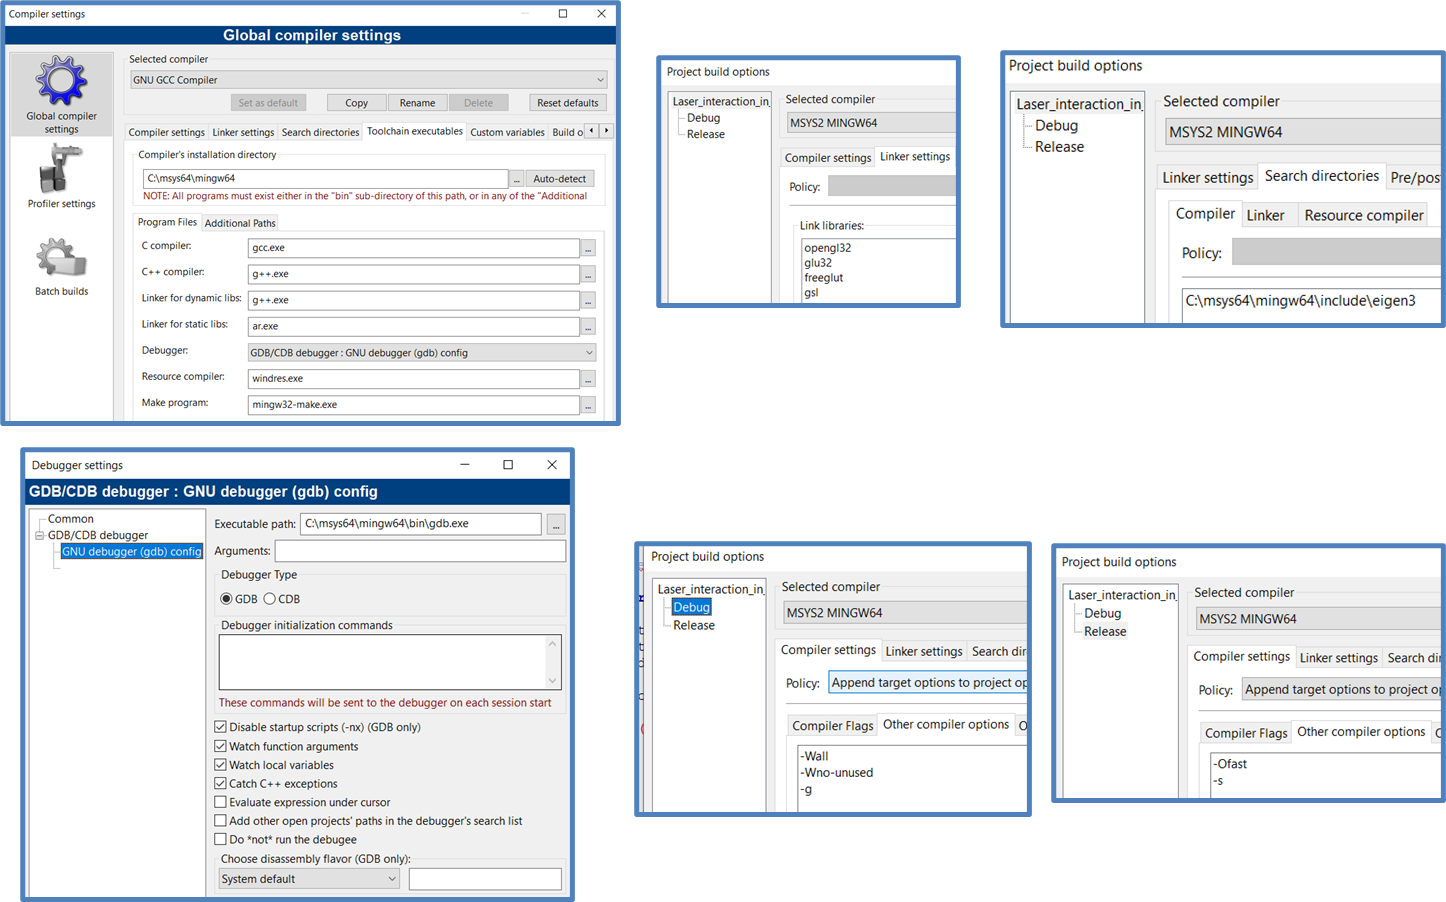
\includegraphics[width=0.7\linewidth]{linker}
	\caption{Example of possible installation (in the case of the simple gsl 1-13). To put either in the Settings/Compiler directory, either in the Project/Build options one.}
	\label{fig:linker}
\end{figure}

	
If you are not at all familiar with CodeBlock I suggest that you follow a small tutorial such as http://www.codeblocks.org/user-manual.

\subsection{64bits}

The steps are:


\begin{enumerate}
	\item  Install last stable version of codeblocks: a mingw-setup.exe binary file from www.codeblocks.org/
	
	It will install the codeblocks in a directory such as C:\textbackslash{}Program Files\textbackslash{}CodeBlocks (see note \footnote{For the 32bits the  mingw-32bit-setup.exe  it will be installed in C:\textbackslash{}Program Files (x86)\textbackslash{}CodeBlocks where the (x86) is here to say that it is a 32bits file but on a 64bits computer. All other "normal" cases will be on C:\textbackslash{}Program Files (that is 32bits on 32system or 64bits files or 64 computer)}).
	

	
\textbf{	Then we need to install useful extra files. This will always be the same idea for all packages (GLUT, GSL, Eigen, ...): put the headers (.h) in an \textbackslash{}include, the .lib (or .a) in a \textbackslash{}lib   and the .dll files of the packages in  a \textbackslash{}bin directory
	 that the code and the compiler will find  for instance by configuring the  project $\rightarrow$ build option.}

Therefore you will hae to adapt the following names for your own installation.
	

\item OPEN\_GL + GLUT (for graphic)


So for example from the github CodeBlocks\_Install repository put

glut32.lib in the sub Directory of Code::Blocks  \textbackslash{}MinGW\textbackslash{}lib

glut.h in \textbackslash{}MinGW\textbackslash{}include\textbackslash{}GL (you may have to create the GL directory).

Finally put the glut32.dll in c:\textbackslash{}windows\textbackslash{}system

\item Eigen Library

To be able to diagonalize an hamiltonian, we need to install the very good library http://eigen.tuxfamily.org
package and unzip it.

Then depending on your location you will have to modify the search directories in the Project Build Options. For me it is
C:\textbackslash{}Program Files\textbackslash{}Common Files\textbackslash{}eigen-3.3.7\textbackslash{}Eigen


\item GNU Scientific Library (GSL)

The simplest way is to install Gsl-1.13-1.exe. then always the same modify from the Search directories in the Project Build Options
the location of the .h files. For me it is
C:\textbackslash{}Program Files (x86)\textbackslash{}GSL-1.13\textbackslash{}include


Then, copy all  .dll (libgsl.dll and libgslcblas.dll and ...) of the GSL installed directory  in Windows\textbackslash{}system


GSL has not .dll and so it is a static linkage. For this you need to create a Global Variable
gsl 
in settings (global variable) of code::blocks with the address where you have installed GSL and add in the 
project $\rightarrow$ build option  $\rightarrow$  search directory  $\rightarrow$ 
linker put: \$(\#gsl.lib)





\end{enumerate}


\subsection{Just run the code}

\subsubsection{Codeblocks configuration}
The main think you have to do to make the code compiling is to make sure that codeblocks find the  files you want (the Eigen, gsl or GLUT ones), the headers (the .h), the library (the .a or .lib files) and the way for windows to handle  (the .dll files).
An example of what should be done is given in Fig. \ref{fig:linker}.


The linker option -Wl,--allow-multiple-definition are here to avoid too many comments. The others such as
-lglut32 (but also
-lopengl32,
-lglu32,
-lgsl)
mean that the compiler has to look for a library file such as libglut32.a or glut32.lib



\subsubsection{speed consideration}
Finally, if wanted, you can increase the speed by looking to  project $\rightarrow$ Build option $\rightarrow$ Compilator and choose your processor  (mine is Intel Core i7). However I almost never find any speed increase (on the contraty so be careful).

For a speed up, you can also use Ctrl+Alt+del and Process $\rightarrow$ to change priority of the program from Normal to high in Windows.


\subsection{Comment on 32 bits more recent version or 64bits codeblocks version.}
\label{32bits}

All this should work if you use a 32 bit computer. For a 64 bit computer you should install the 64bit GSL version and the 64bits codeblocks version


\begin{enumerate}
\item 64bit installer (MSYS2 MinGW)

The best (because Cygwin leads to a lot of problem) is to get an installer of  MSYS2 MinGW w64-bit and run it. Then using the package manager (pacman) do:
\begin{itemize}
	\item  pacman -Syu 
	\item pacman -Syu base-devel (then make the selection that avoids pacman: typically 1-39,41-58 that avoids pacman at number 40 in this example)
	\item	pacman -Syu mingw-w64-x86\_64-toolchain (then choose all)
\end{itemize}


\item 64bits GSL 


Retrieve the last GSL folder for example gsl-2.6, unzip it for instance in C:\textbackslash{}msys64\textbackslash{}home\textbackslash{}daniel and install with MSYS2 :
\begin{itemize}
	\item  cd gsl-2.6
	\item % ./configure --prefix=C:/msys64/mingw64 (be careful, it's a space then twice - in front of prefix). If this does not work try just 
	./configure
	\item make
	\item make install
\end{itemize}

Obviously you then need in the codeblocks project to put the proper
Gsl : 

- Settings / Global Variables / base: write the path of the main folder of gsl in msys. 		For example C:\textbackslash{}msys64\textbackslash{}home\textbackslash{}Daniel\textbackslash{}gsl-2.6

- Project / Build options... Select the right compiler (at the very bottom of the list)

- Project / Build options... / Search directories: fix the path For example
 C:\textbackslash{}msys64\textbackslash{}MinGW64\textbackslash{}include
 
 
 
 
 \item   64bits latest Codeblocks
 
  So you should download the mingw-setup.exe codeblocks binary file from www.codeblocks.org/
 or if you want the
 newest codeblocks version. You can download the last version "out" of Nightly built: http://forums.codeblocks.org/index.php/board,20.0.html
 that is download three .7z files, unzip them (you need 7Zip) in CodeBlocks directory by replacing all the old files with them. 
 
 
 \item C++ 64bits compiler
 
 The last version of code blocks has a 64bit compiler so this is not needed
 
 
 
 You may need to change to Compiler in codeblocks For this go to Settings/compiler/ and select the default compiler and copy, give a name, for example MSYS2 MINGW64
 Go to Settings/compiler/GlobalCompilerSettings/ToolchainExecutables" to set the path of MinGW64 installed at the beginning: C:/msys64/mingw64.
 Put the right file names in the "program files" tab of executable toolchain: change all names (exemple x86\_64-w64-mingw32-gcc.exe instead of mingw32-gcc.exe) except the one for make (you will find  the names in the bin folder of mingw64).
 
 
 

\item GLUT  



All this works but the onyl problem is GLUT that has some issues that needs also to be fixed because it is intrinsically  32bit.
The best is probably to use  freeglut from https://www.transmissionzero.co.uk/computing/using-glut-with-mingw/

First it may be wise to know that 32bits dll in a 64bit system should go to  c:\textbackslash{}windows\textbackslash{}SysWOW64. All other standard case go to System32 (I know this is confusing but comes from histrorical reasons like (x86) = 32nits and (x64)=64 bits).





Run the Command Prompt in administrator mode (type "cmd" on the start menu + click the Run as administrator" option) then run: \%windir\%\textbackslash{}System32\textbackslash{}regsvr32.exe /u glut32.dll
\ and \
\%windir\%\textbackslash{}SysWOW64\textbackslash{}regsvr32.exe /u glut32.dll

\end{enumerate}


\subsection{Parallelization by means of OpenMP}

Additionally, the execution of the code, especially parameter scans can be accelerated by parallelizing the program onto all CPUs available on the according computer in use. The number of CPUs or threads can be found for example in the Windows Task Manager (In the following it will be described for a quad-core processor, in case of a different number of available CPUs the number 4 in the following example of course has to be adjusted accordingly.).

For the purpose of parallelization the application programming interface called OpenMP (Open Multi-Processing) has to be configured in the corresponding CodeBlocks installation. Additionally the two files \textit{main\_Laser\_Cooling.cpp} as well as \textit{Liste\_Param.h} have to be modified accordingly. We detaield in great details how to do it if needed.

Step by step, the configuration should be carried out in the following way:

\begin{enumerate}
	\item Modification of CodeBlocks compiler settings:
	
	\begin{itemize}
		\item Add the flag \textit{-fopenmp} under \textit{Settings} $\rightarrow$ \textit{Compiler} $\rightarrow$ \textit{Global compiler settings} $\rightarrow$ Tab \textit{Compiler settings} $\rightarrow$ Sub-Tab \textit{Other compiler settings}
		
		\item Add the flags \textit{-lgomp -pthread} under \textit{Settings} $\rightarrow$ \textit{Compiler} $\rightarrow$ \textit{Global compiler settings} $\rightarrow$ Tab \textit{Linker settings} $\rightarrow$ Sub-Tab \textit{Other linker options}
		
		\item Add the path \textit{\path{C:\msys64\mingw64\lib\gcc\x86_64-w64-mingw32\10.2.0\include}} (or respective path to the folder containing the header file \textit{omp.h}) under \textit{Settings} $\rightarrow$ \textit{Compiler} $\rightarrow$ \textit{Global compiler settings} $\rightarrow$ Tab \textit{Toolchain executables} $\rightarrow$ Sub-Tab \textit{Additional Paths}.
	\end{itemize}
	
	\item Modifications in \textit{main\_Laser\_Cooling.cpp}:
	
	The idea for parallelization here is to run one instance of the code on each available CPU core but with different simulation parameters, such as laser power, detuning, bandwidth or any other variable which is set in the \textit{Liste\_Param.h}. This is achieved by creating several \textit{Liste\_Param.h} files, namely each per core, defining the parameters for this instance. Therefore the following changes have to be made in the main code file \textit{main\_Laser\_Cooling.cpp}:
	
	\begin{itemize}
		\item First of all, \textit{include <omp.h>} has to be included right in the beginning of the file in order to include the OpenMP header file.
		
		\item Under \textit{\/***  NOM DES FICHIERS ***\/} the new variables and files for the separate instances have to be defined and packed into vectors. Code examples in case of the implementation on a quadcore CPU and with the four new parameter files called \textit{Liste\_Param1-4.h} can be found in Figures \ref{fig:Parallelization_Mod1_main.cpp} and  \ref{fig:Parallelization_Mod2_main.cpp}.
		
		The references to the according non-vector variables which have been used previously in the code have to commented of course. Namely these are the following lines:
		
		\textit{nom\_sortie\_donnees\_string = data.SParam("nom\_sortie\_donnees");}
		
		\textit{nom\_sortie\_rate\_string = data.SParam("nom\_sortie\_rate");}
		
		\textit{nom\_sortie\_donnees = nom\_sortie\_donnees\_string.c\_str();}
		
		\textit{nom\_sortie\_rate = nom\_sortie\_rate\_string.c\_str();}
		
		\begin{figure}[h]
			\centering
			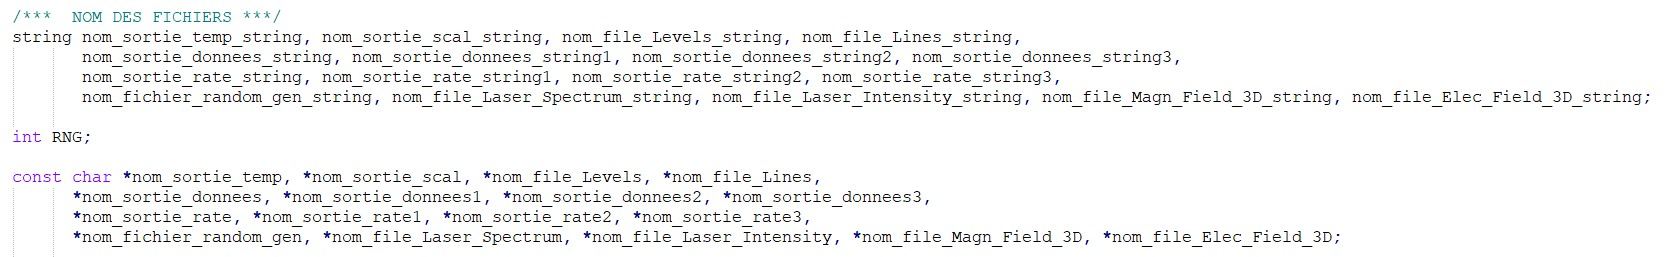
\includegraphics[width=0.9\linewidth]{Modifications main_Laser_Cooling 1.jpg}
			\caption{Definition of new variables for parallelization.}
			\label{fig:Parallelization_Mod1_main.cpp}
		\end{figure}
		
		\begin{figure}[h]
			\centering
			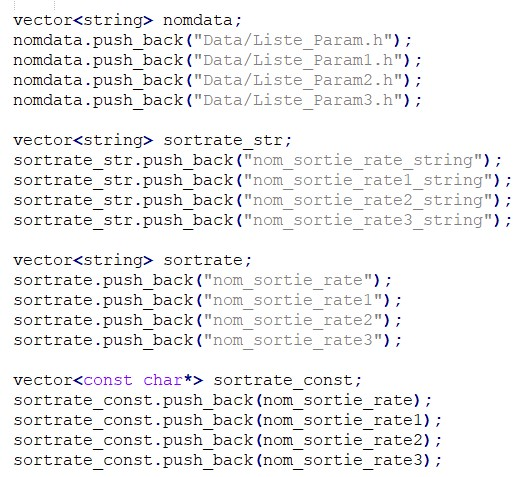
\includegraphics[width=0.35\linewidth]{Modifications main_Laser_Cooling 2.jpg}
			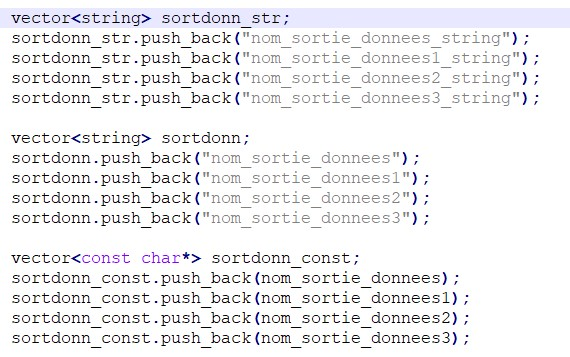
\includegraphics[width=0.35\linewidth]{Modifications main_Laser_Cooling 3.jpg}
			\caption{Definition of new variables for parallelization.}
			\label{fig:Parallelization_Mod2_main.cpp}
		\end{figure}
		
		\item Finally, the main program has to be enclosed in a control sequence in order to initialize the instances one each of the cores and while looping over the different parameter files. This control sequence is introduced by inserting the three lines shown in Figure \ref{fig:Parallelization_Mod3_main.cpp}.
		
		\begin{figure}[h]
			\centering
			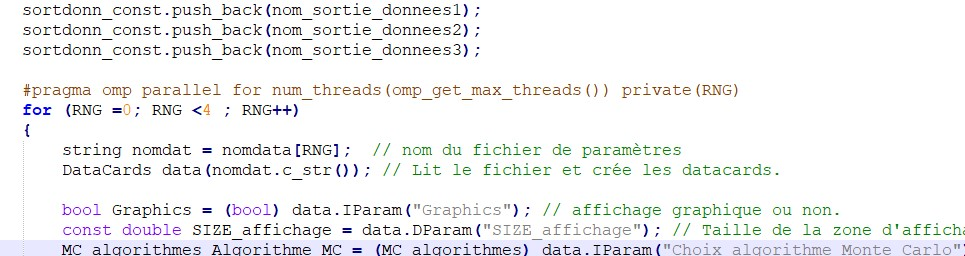
\includegraphics[width=0.65\linewidth]{Modifications main_Laser_Cooling 4.jpg}
			\caption{Introduction of additional control sequence.}
			\label{fig:Parallelization_Mod3_main.cpp}
		\end{figure}
		
		Of course this loop needs to be closed finally, as shown in Figure \ref{fig:Parallelization_Mod4_main.cpp} for example.
		
		\begin{figure}[h]
			\centering
			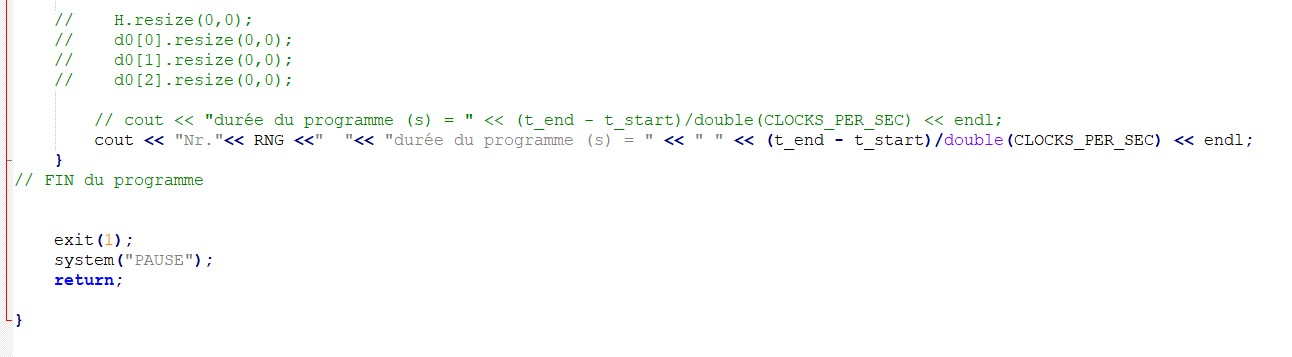
\includegraphics[width=0.8\linewidth]{Modifications main_Laser_Cooling 5.jpg}
			\caption{End of additional control sequence.}
			\label{fig:Parallelization_Mod4_main.cpp}
		\end{figure}
		
	\end{itemize}
	
	\item Modifications in \textit{Liste\_Param.h}:
	
	Each of the four parameter files has to be adjusted by adding the additional output files here as well under \textit{	NOM\_FICHIERS 	 } and by defining their names, for example in the following way: 
	
	\textit{\path{@nom_sortie_donnees} \ \ \ \ \path{Data/donnee_Mol.dat}} \\
	\textit{\path{@nom_sortie_donnees1} \ \ \ \ \path{Data/donnee_Mol1.dat}} \\
	\textit{\path{@nom_sortie_donnees2} \ \ \ \ \path{Data/donnee_Mol2.dat}} \\
	\textit{\path{@nom_sortie_donnees3} \ \ \ \ \path{Data/donnee_Mol3.dat}} \\
	\textit{\path{@nom_sortie_rate} \ \ \ \ \path{Data/sortie_rate.dat}} \\
	\textit{\path{@nom_sortie_rate1} \ \ \ \ \path{Data/sortie_rate1.dat}} \\
	\textit{\path{@nom_sortie_rate2} \ \ \ \ \path{Data/sortie_rate2.dat}} \\
	\textit{\path{@nom_sortie_rate3} \ \ \ \ \path{Data/sortie_rate3.dat}} \\
	\textit{\path{@nom_fichier_random_gen} \ \ \ \ \path{Data/random_gen.txt}} \\
	\textit{\path{@nom_sortie_donnees_Data} \ \ \ \ \path{Data/data_card1.dat}} \\
	
	
\end{enumerate}

% https://instincttechies.blogspot.com/2013/06/how-to-use-openmp-in-codeblocks.html
% https://www.youtube.com/watch?v=IQdZwIM8r_c










\section{Short overview}

\subsection{Overview of the Program}

You do not need to know the code in detail, but an overview of its C++ structure is given in the Figures  \ref{fig:Class} and \ref{fig:Program_evolution}.


\begin{figure}
	\centering
	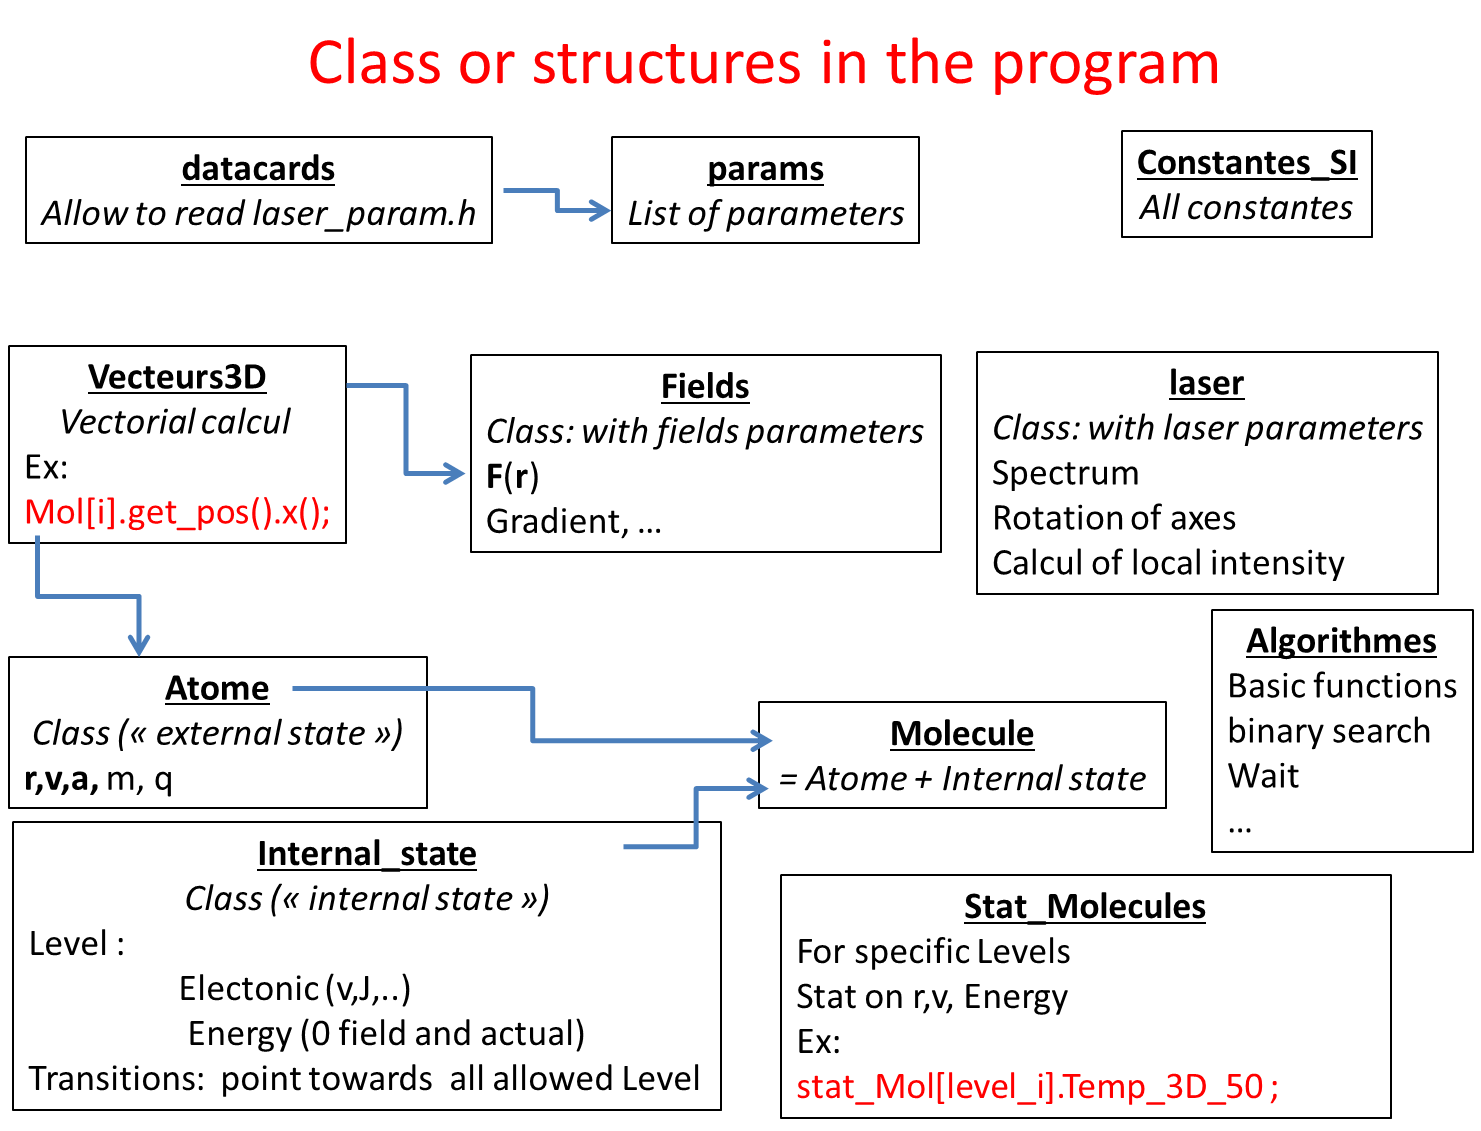
\includegraphics[width=0.7\linewidth]{classes}
	\caption{Schematic of the structure and some basics functions used by the code. The blocks are the different files (.cpp or .h) present with their names in bold and an quick explanation of what they do.}
	\label{fig:Class}
\end{figure}


Figure \ref{fig:Class} gives the list of the basic structure or classes used such as lasers or fields. Molecules are just seen as Levels, Lines and their positions and velocities.

Figure \ref{fig:Program_evolution} is the core of the code with the main evolution summarized in the Main\_laser\_cooling.cpp program, that is usually the only code that you may have to modify (with the output one: sortie\_donnee).
As you see the code as still some French in it such as:

\begin{itemize}
	\item donnee = data
	\item affichage = plot
	\item sortie = output
	\item champ = field
 \end{itemize}


 

\begin{figure}
	\centering
	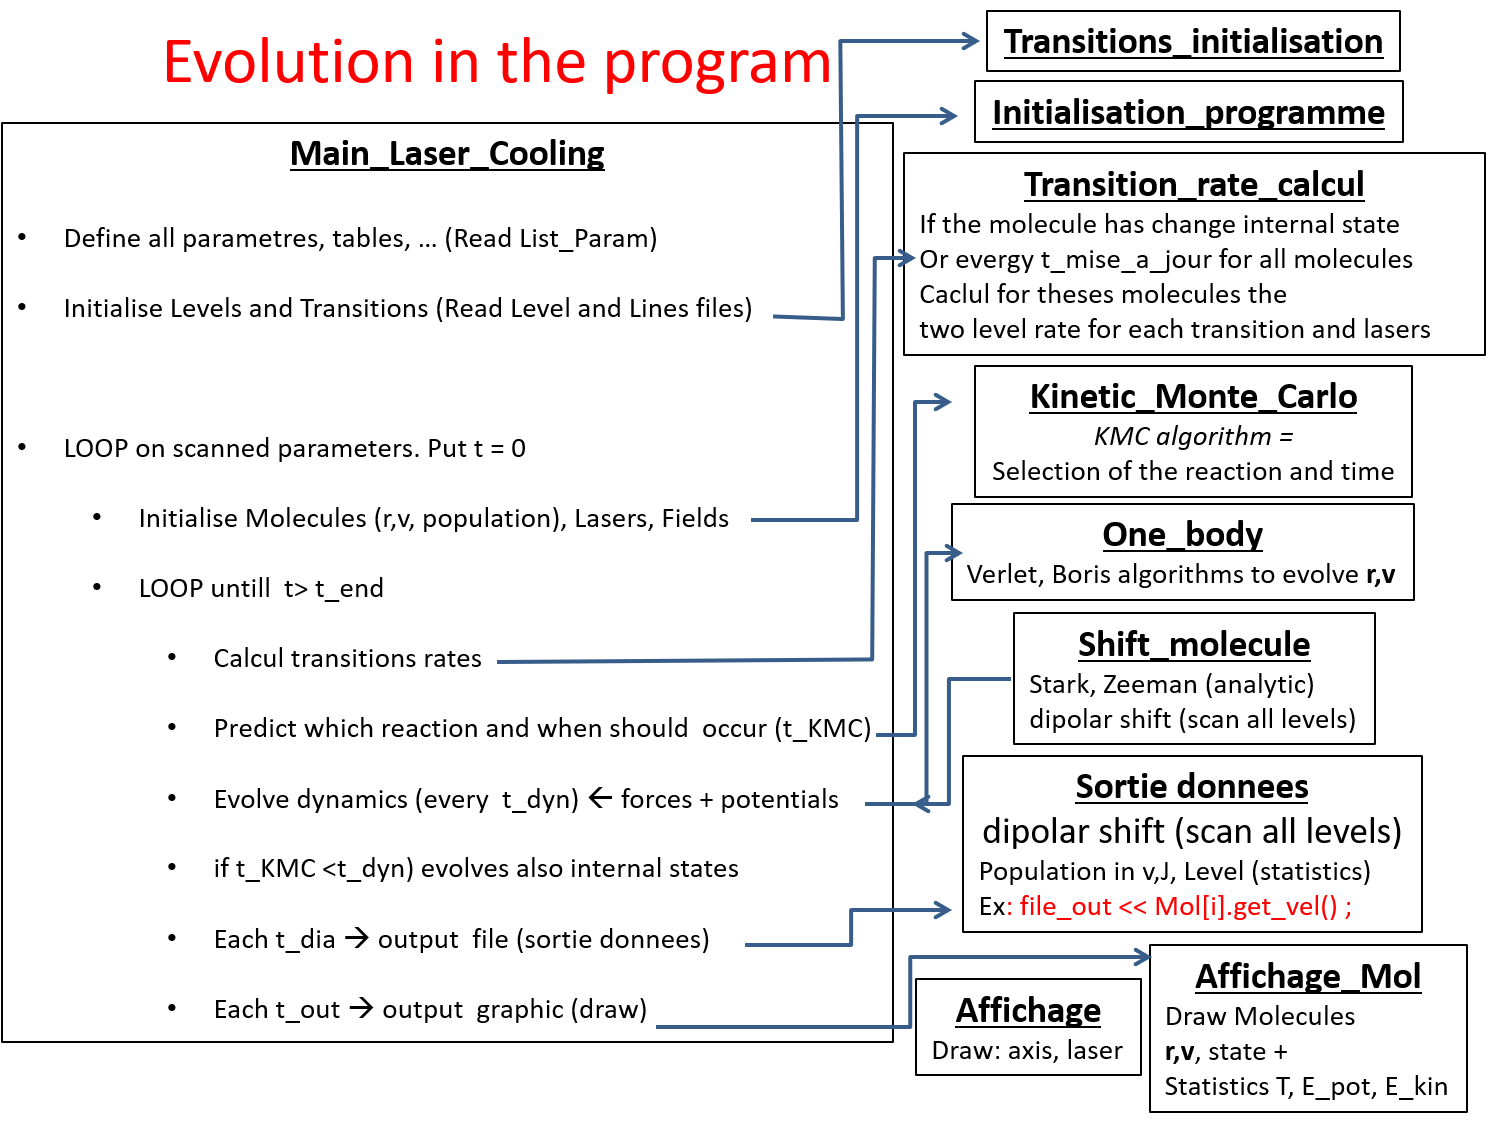
\includegraphics[width=0.7\linewidth]{evolution}
	\caption{Schematics of how the code evolve its time. The blocks are the different files (.cpp or .h) present with their names in bold and an quick explanation of what they do.}
	\label{fig:Program_evolution}
\end{figure}





\subsection{graphics}


Once run. You will see two screens appearing as shown in figure
\ref{fig:picture}. 



\begin{figure}
	\centering
	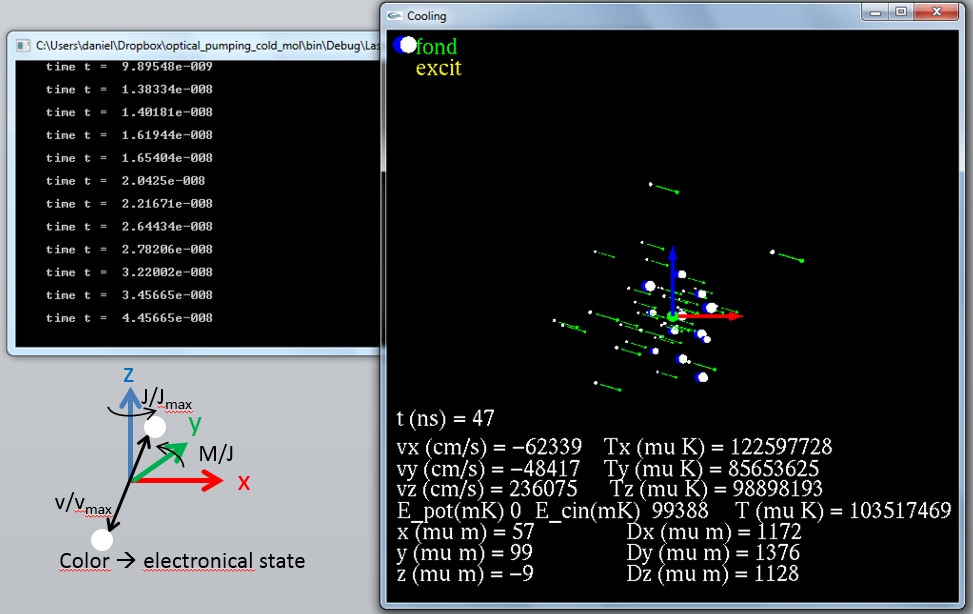
\includegraphics[width=0.7\linewidth]{picture}
	\caption{Snapshot (screen capture) of the code.}
	\label{fig:picture}
\end{figure}



If you do not want the graphics you have to change the option in Liste\_Param file.
Some parameters like the screen size are directly part of the code but other ones like size of view of the sample are part of Liste\_Param.


For now the graphics do not indicate the lasers locations but show the particles behavior at every time steps, set by the parameter
$@${}dt\_out of Liste\_Param

The graphics (uses OPEN\_GL library for 3D plotting) represent the particles with the following choices:
\begin{itemize}
	\item Red arrow along x, green along y and blue along z (gravity is along -Oz) to see the origin and orientation of the view.  Global screen rotations are possible in Liste\_Param, the usual one puts gravity down, but if no rotation is performed we would have x toward the right, y up and z toward the screen.
	\item Molecules are represented like diatomic molecules (a line connecting 2 balls) 
and depend of their ro-vibronic level and mass.
	The length is proportional to the vibrational quantum number $v$, the angle in $x y$ is proportional to the rotational quantum number $J$ and the angle in $x z$ is proportional to its projection (along the local field axis) $M$. 
	Then the ball size and the color reflects the molecule and its state: Ground state are green, excited state are yellow, dead (photodetachment, ionization, annihilation)	are blue (and antiprotons are olive).
	
\end{itemize}



Then some statistical data are given like the temperature, positions and velocities of the laser cooled molecules.
As well as the temperature of the second species (if they exist). 
Finally the total energy of all molecules is given (it should be conserved in absence of laser cooling).


\subsection{Output: Export data in files}

In addition to the graphics output we have several others possible outputs.

Mainly Sortie\_donnee\_pop\_vJ gives the population in each $v,j$ levels or simply  Sortie\_donnee\_pop\_v gives the population in each $v$ levels. But the standard one is
Sortie\_donnee that gives useful data such as positions, velocities or temperatures.

The current example  Sortie\_donnee (call in main\_Laser\_cooling.cpp  in "(t $>$= t\_dia)" section)
gives for each diagnositic time: the parameters that you scan, the time, the position (x,z) and v\_z.

{\bf You Should probably modify those outputs for your own purpose.}
Use the comment lines to inspire you for your own choice.


Finally you can stop the code to run by pressing CTRL+C after if you want to stop before the end or to avoid producing too big files.

\section{Input files}


The code requires source input files 
(their locations and names are defined in Liste\_Param). The files are the following:

\begin{enumerate}
\item Liste\_Param.h (it has to have this exact name)

Contains all relevant parameters such as number, temperatures, locations of the particles, lasers parameters and some output properties and algorithm choices.
The location of the files are also given in $@${}nom\_file\_Levels,   
$@${}nom\_file\_Lines    or $@${}nom\_file\_Laser\_Spectrum  



	\item "Levels".
	
	Contains informations about the levels of the chosen particle (BaF, Cs$_2$, NH, Cs, CO, Ps, ...). The basic informations are the energy levels and their linear and quadratic Zeeman (and eventually Stark) shifts.
	
	\item "Lines" .
	
	Give the dipole transition strength between two levels.
	
	\item "Laser Spectrum[i]"
	 
	It is optional (if not present no laser attenuation is taken into account and the laser is "normal"). But it can be used to create spectral shaping of a laser.
	

 
\end{enumerate}


ALL FILES SHOULD NOT contain a return line neither an extra character, like a space, at the end!




\begin{figure}
	\centering
	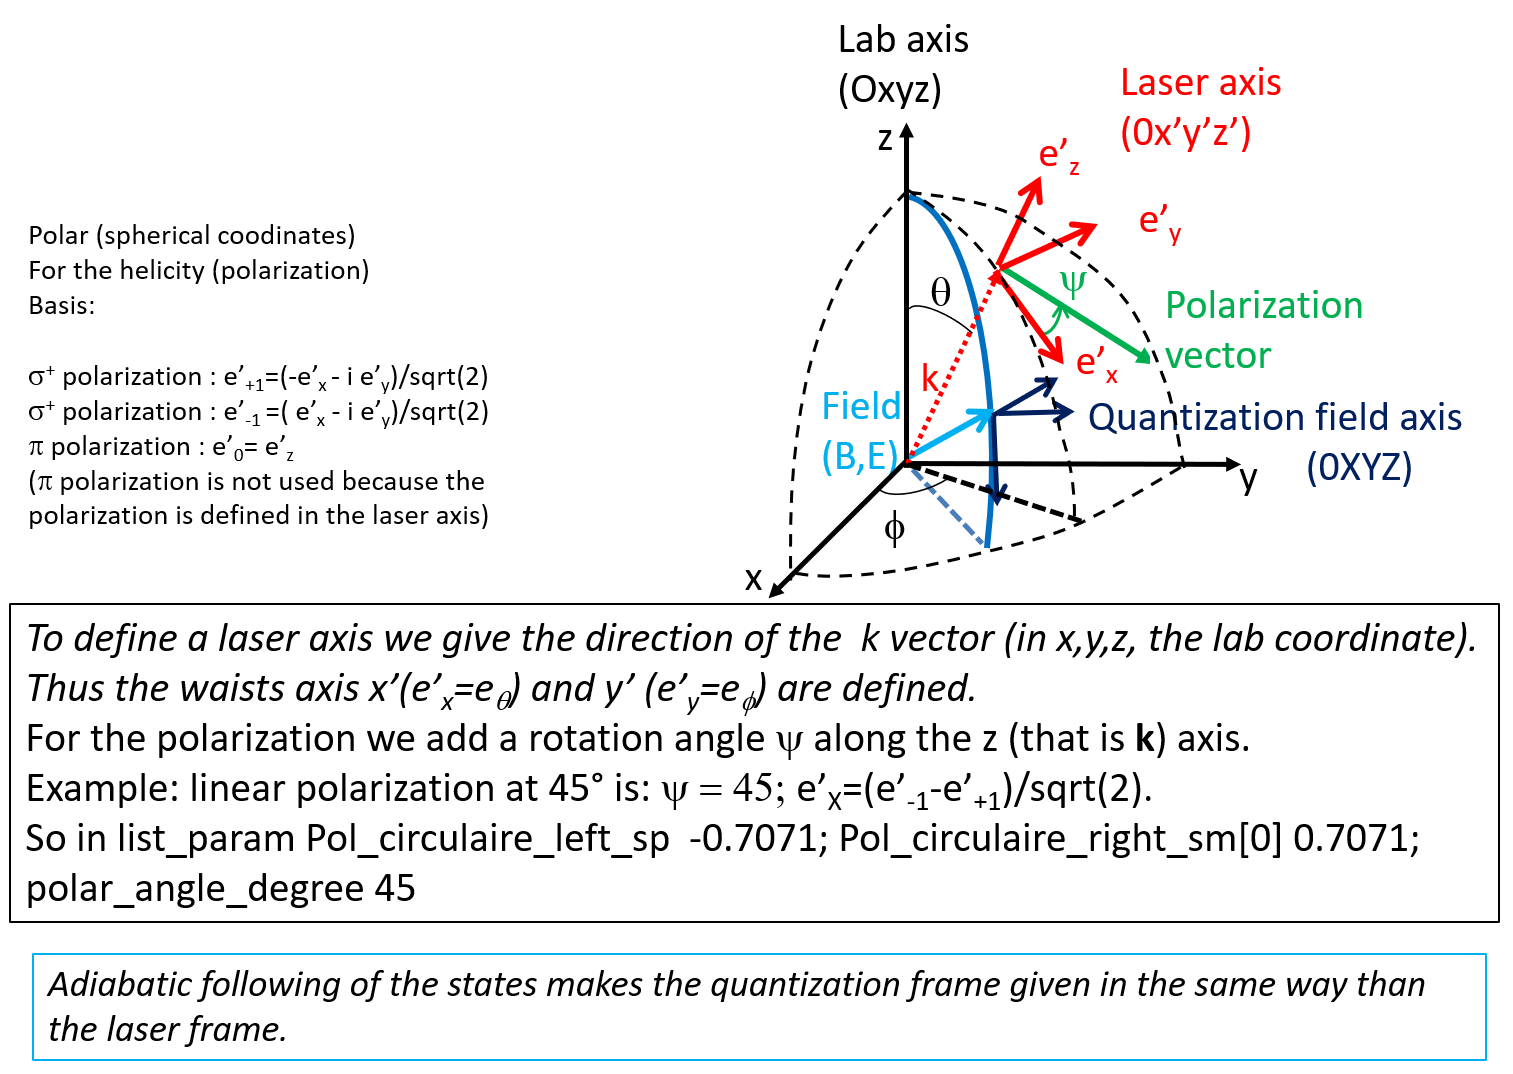
\includegraphics[width=0.7\linewidth]{laser_axis_polarization}
	\caption{Definition of the differents frame: laser axis (for the polarization basis),  field axis (that is the quantization because we assume adiabatic following of the states) and lab fixed frame. 	To go from the lab fix frame to the laser axis one 	 a first rotation is by an angle $\phi$ about the $z$-axis then a second rotation is by an angle $\theta$  about the new $y$-axis
	}
	\label{fig:laseraxispolarization}
\end{figure}



The structure of the files have been chosen because it is the one given by the Pgopher program: PGOPHER, a Program for Simulating Rotational Structure, C. M. Western, University of Bristol, http://pgopher.chm.bris.ac.uk. See Journal of Quantitative Spectroscopy \& Radiative Transfer 186 (2017) 221, where Pgopher is described.

A more detail description of all files is now given.

\subsection{Liste\_Param} 

Liste\_Param.h contains:
\begin{itemize}
	\item Particles parameters: numbers, type, temperatures, initial positions and velocities
	\item Graphics: size and angle of the field of view,  time for each output.
	\item Fields. Usually given in 3D up to the second order. We can put Helmholtz coils for the magnetic field. For now we can have a trapping magnetic or electric field but not both. With the exception of a Penning trap where the electric field acts on the charge but is supposed to not produce internal energy shifts.
	\item Laser beams:  waist sizes and positions, polarisations, powers, linewidths, wavelengths, spectral shapes (Lorentzian, Gaussian, comb lines) and possible coherence (intensity interference to create optical lattice) between them.... The polarization could be purely circular (left=$\sigma^+$ or right=$\sigma^-$) or linear and are defined using the laser propagation axis and a rotation angle cf Fig. \ref{fig:laseraxispolarization}. Linear polarizations are thus possible but (to be checked..) then no interference effects are taken into account. Other 'fictuous' laser types can be invented in order to take into account other rates (such as collisional, field ionization, ...)
		\item Algorithm parameters: evolution time and steps. Among them we have 
the Kinetic Monte Carlo, the First Reaction Method or the less accurate but faster Random Selection Method or even the Fast Rough Method for the internal state. Verlet or Boris-Buneman for the external motion but with different types: either using the analytical acceleration (and no dipolar force) either using gradient of the potential (the epsilon "size step" has to be manually optimized). A N-body algorithm is also implemented. 
  
\end{itemize}


In principle all parameters are in SI units. If not, the name suggests the value such as Gamma\_L\_MHz or Energy\_cm because all energies are in cm$^{-1}$.


All parameters have their name staring with $@$ symbol followed by their value (so no symbol $@$ should be use in this file except for this purpose).


A loop on the parameters values can be done if the parameters names are written with a
$@${}SCAN\_ prefix and a "true" value between 
BEGIN\_OF\_FITPARAMS
and 
END\_OF\_FITPARAMS
at the end of Liste\_Param.h file.




If needed, a new parameter can be added in the file, and then used, in some files of the program using the sentence
 params.LocateParam("Nom\_Parametre")-$>$val
that takes its value.




\subsection{Levels}


The name of the file can be chosen as wanted but then put in the Liste\_Param.h file.

The columns of the file are the following:

	\bigskip
	
 \textbf{ Manifold	2M	Sym	\#	population  }	v 	2J	2N	2$\Omega$	 \textbf{ E$_{\rm cm}$	$\Delta$	C}
		\bigskip

Columns are separated by tabulation. Points (not coma) are used for decimal separations.


 \textbf{ manifold, 2M, \#, Sym  are the only data used to label a Level}. Thus v, 2J, 2N or 2$\Omega$ are extra data and are here only for a better understanding of the file. They can also be used for an output of the data.

The detail of the columns are(in bold the data that should absolutely be correct):

\begin{itemize}
\item 	 \textbf{Manifold}: usually 0 means ground electronical level, 1 is for an excited electronical level, 2 for another one ... Negative values can be used for a "dead" level such as one in a continuum (photo-ionization -1, photodetachement -2, or annihilation -3).
	
	\item 	 \textbf{2M}: where  M is the projection of the total angular momentum. We note 2M and not M to be able to use integer in the code for M=1/2 for instance.
	In the code the particle will be assumed to always follow (adiabatically) the local quantification axis given by the local field.

<<<<<<<< Updated upstream:User Guide/User Guide Laser Cooling_old.tex
{\it If you want to simulate states without sub-structure like pure ro-vibrational transition in zero field you coudld impose $M$=0 for all states and use $\pi$ laser polarization.}	
========
{\it If you want to simulate states without sub-structure like pure ro-vibrational transition in zero field you could impose $M$=0 for all states and use $\pi$ laser polarization. Another common "trick" is to create "dead" levels with proper dipole transition for an annihilation event that will be mostly treated as a spontaneous emission event}	
>>>>>>>> Stashed changes:User Guide/User_Guide_Laser_Cooling_v2.4.tex
	
\item 	 \textbf{Sym}:  Originally it was the parity of the state but this not the case but it should be +1 or -1 to design  bound states and 0 for an continuumm state (that is above the continuum threshold such as for photodetachment or photoionization).

\item 	 \textbf{\#}: "number" of the state. It lifts the degeneracy between levels having the same 3 parameters: manifold, 2M and \#. Usually it is ordered (0,1,2, ...) by energy  but for the vibrational levels you could add 10000v to keep trace of it.

\item 	 \textbf{population}: This is proportional to the initial population in the levels (that will be taken randomly at the beginning of the run). The sum should not have to be 1.


\item v: vibrational level. As said previously this is not used by the code except may be for some output data. 

\item 2J: J = total angular momentum (F if nuclear spin present) 

\item 2N: N = rotational angular momentum, including L (L=electron orbital angular momentum). 

\item 2$\Omega$ : $\Omega$ = Projection of J along the molecular axis. 

 
\item \textbf{E$_{\rm cm}$}: energy of the level in cm$^{-1}$. For a continuum state, we put the energy of the threshold, like that we can test if the laser transition reach the continuum or not (but we assume a cross section independent of the energy).

\item \textbf{$\Delta$ and C} give the energy shift of the level under an electric or magnetic field $F$. 

The formula is $E_{\rm cm}(F)= {E_0}_{\rm cm} + {\rm sign}(C) [-\Delta/2+\sqrt{(\Delta/2)^2+(C F)^2}]$.
Thus if $\Delta = 0$ we have a linear variation $E(F)= E_0 + C F$. 
Thus, for the magnetic field case, units are  cm$^{-1}$/Tesla for $C$. A magnetic moment of 1 $\mu_{\rm Bohr}$ correspond to a value for $C$ of  0.4668645 cm$^{-1}$/Tesla.


\end{itemize}

If needed, an option exists (is\_File\_FC in Liste\_Param) in order to automatically produce new Levels and Lines files from a file containing only $v_X=0 \rightarrow v_A =0$ transition by reading  extra Franck-Condon and vibrational and rotational constant files.



\subsection{Lines}

The lines file can content more lines than used by the Level file. In this case the program only read the useful ones.
	
	The columns (separated by tabulation) of the file are the following:
	

	
	\bigskip
	
 \textbf{UpperManifold	2M'	Sym'	\#'	LowerManifold	2M''	Sym''	\#''}	$\Delta_E$	Intensity	E$_{\rm upper}$	E$_{\rm lower}$	 \textbf{Strength}	 
	
\bigskip

 \textbf{The first 4 columns design the upper level $|1\rangle$ and the second 4 the lower level $|0\rangle$.
So they have to be the same as in the Level file!}

  The last 5 columns give informations about the transitions between these levels.
But  \textbf{only the last column (Strength)	  is used by the code}. However, usually they are composed on:

\begin{itemize}


\item $\Delta_E$: energy difference between the 2 states $|1\rangle$ and $|0\rangle$.

\item Intensity: Einstein coefficient = spontaneous emission rate of the transition (this is not the total decay rate of the state $|1\rangle$, because it can decay to several levels).

\item E$_{\rm upper}$: energy in cm$^{-1}$ of the upper state $|1\rangle$.

\item E$_{\rm lower}$: energy in cm$^{-1}$ of the lower state $|0\rangle$.

\item  \textbf{Strength}: $S_{\rm pol}=d_{\rm axe}^2/3$, where $d_{\rm axe}$ is the dipole (in Debye) of the transition along the polarization axis that authorize the transition between the sum-Zeeman levels).  This notation was used due to historical reasons linked to Pgopher.

So   A=Intensity = $\Gamma = 3 S_{\rm pol} C_{{\rm Debye},s} E_{\rm cm}^3$ 
with  $C_{{\rm Debye},s} = (8\times 10^6 \pi^2 c^3 {\rm Debye}^2 )/(3. \varepsilon_0 c^3 \hbar) = 3.13618932 \times 10^{-7}$ is the conversion from the dipole (in Debye) to the Einstein's coefficient A  (s$^{-1}$) for an energy in cm$^{-1}$.



\end{itemize}



<<<<<<<< Updated upstream:User Guide/User Guide Laser Cooling_old.tex
For an continuum transition (so with Sym' = 0), the idea to treat it, is to put a "fake" level: the energy should be just at the ionisation threshold (thus the program can test if the laser wavelength is enough to ionize). But, in this case the $S_{\rm pol}$ column is  not $d^2/3$ but $\sigma/$cm$^2$ which is the ionization cross section in cm$^2$.
========
For an continuum transition (so with bound\_state' = 0), the idea to treat it, is to put a "fake" level: the energy should be just at the ionisation threshold (thus the program can test if the laser wavelength is enough to ionize). 
There is only one constant value for the dipole (so for the cross section), no wavelength dependence is included so you have to choose the one adapted to your lasers.
>>>>>>>> Stashed changes:User Guide/User_Guide_Laser_Cooling_v2.4.tex




\subsection{LASER\_SPECTRUM} 
 
This file is used only if you want to  shape spectrally a laser.  If you do not create such a file a default one (containing only one line: 0 1) is created which does not affect the laser intensity.


The code reads a file one file per laser (number).
Laser\_spectrum[i] for laser number i+1
that contains 2 columns: E$_{\rm cm}$  (Energy in cm$^{-1}$) and Attenuation (intensity attenuation coefficient).


When a transition should occur at the energy  $E_{\rm cm}$. 
The program look in this file for the line $i$ such as  $E_{\rm cm}[i] \leq E_{\rm cm} < E_{\rm cm}[i+1]$ and then it takes the corresponding value 
Attenuation$[i]$. This will be the multiplicative factor for the laser intensity for this transition energy.
So in summary the energy in the file is the energy just below yours and the intensity would thus just be multiplied by the amplitude factor.


<<<<<<<< Updated upstream:User Guide/User Guide Laser Cooling_old.tex
========
\begin{figure}
	\centering
	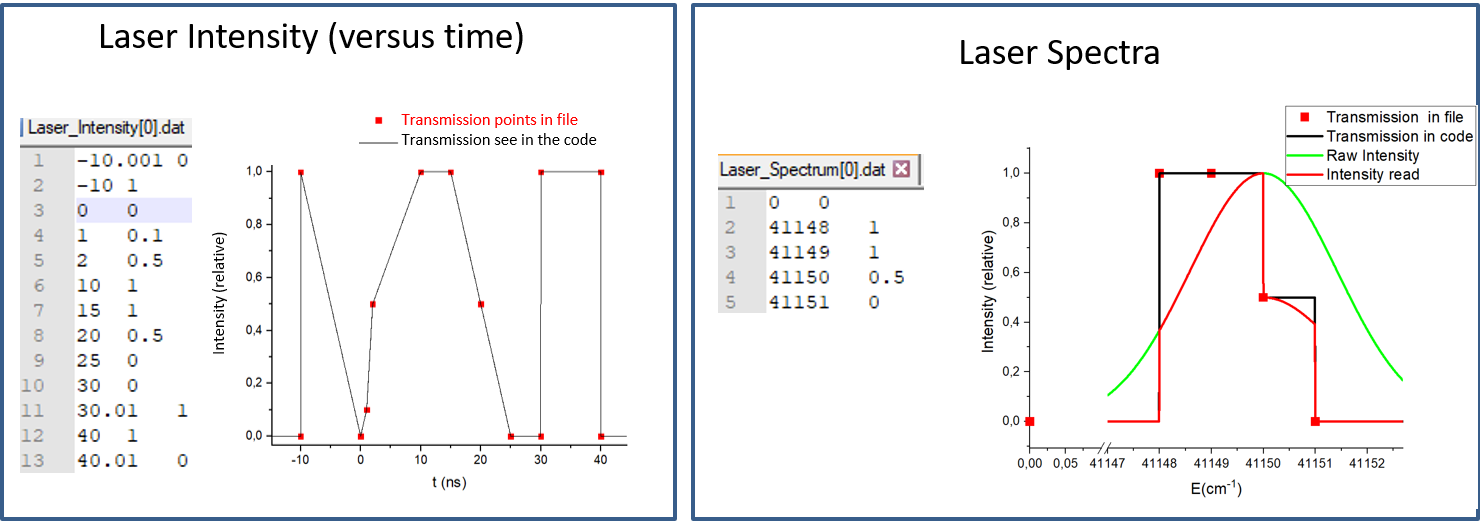
\includegraphics[width=1\linewidth]{shaping}
	\caption{Shaping examples. Left  shaping for the laser intensity versus time: the code (solid black line) interpolate linearly between (red) points, if the point is before or after the points we kept the nearest value. Right: shaping for the laser spectrum: the value of the interpolation is the lower one in the file (no interpolation between red points). The example illustrate a gaussian laser, 100 GHz broad. In Red is the final (relative) intensity.}
	\label{fig:shaping}
\end{figure}



\subsection{LASER\_INTENSITY} 

This file is used only if you want to  shape the intensity in time for a given a laser. 
It is important to know that this is a pure intensity effect, no (Fourier-Transform) spectral effect is liked to it (so we can not create a broadband femtosecond laser just using this for instance).
 If you do not create such a file a default one (containing only one line: 0 1) is created which does not affect the laser intensity.


The code reads a file one file per laser (number).
Laser\_intensity[i] for laser number i+1
that contains 2 columns: $t_{\rm ns}$  (time in ns) and transmission $T$ (intensity transmission coefficient).


When a transition rate is calculated at time $t$, the program look in this file for the line $i$ such as  $t_{\rm ns}[i] \leq t < t_{\rm ns}[i+1]$ and then it interpolate, at first order, the corresponding value between
$T[i]$ and $T[i+1]$. So $A$ is the transmission value:
$T = T[i] + \frac{T[i+1]-T[i]}{t[i+1]-t[i]}(t-t[i])$. After the last point the intensity is kept constant, so it is wise to put $T=1$ (or $T=0$) as last point.
This will be the multiplicative factor for the laser intensity.

>>>>>>>> Stashed changes:User Guide/User_Guide_Laser_Cooling_v2.4.tex


\section{Troubleshooting}


Figures \ref{fig:Program_evolution} is the core of the code with the main evolution summarized in the Main\_laser\_cooling.cpp program, that is usually the only part of the code that you have to modify (with the output one: sortie\_donnee).


If the program does not run for the first time it is usually a problem of links and library in Code::Blocks.

But if it usually runs but then bug after some modifications it is 90\% due to an error in the input files: levels or lines!


For debugging use the debugger in the Debug file. But you can also use  Sortie\_rate  which gives all rates, or Sortie\_donnee\_etat\_int\_simple that gives the list of levels, and that are commented on Main\_Laser\_Cooling. You have also Sortie\_laser\_spectrum to check the laser spectrum you make or Sortie\_transition to check the transition per

\textcolor{red}{The best way to debug is to use a simple two level system and to look for the rates to understand if they are as expected. 95\% of the time the problems comes from the Levels or Lines files}


\subsection{CodeBlocks problems}

If you have not strictly followed the rules you might have the following problems!!


If Code::Blocks is installed in the  C: directories but you have put your project in D: 
this does not work.
Thus, you have to put in
"Settings" $\rightarrow$ "Compiler and Debugger" $\rightarrow$ "Toolchain executeables" $\rightarrow$ "Program files"
some link.
For instance modify "mingw32-g++.exe" in "C:\textbackslash{}MinGW\textbackslash{}bin\textbackslash{}mingw32-gcc.exe" 
in the "linker for dynamics libs:"...

More generally the problems are almost always coming from a bad links.
 You can specify them for your global environment or just for your project.

For global environment :
\begin{itemize}
	\item Menu Settings/Compiler and debugger
\item In the Global compiler settings, select the Search directories
\item Add the required paths for compiler and linker.
\end{itemize}


For your project :
\begin{itemize}
	\item  Right click on the project then select Build options
\item Select the Search directories
\item Add the required paths for compiler and linker.
\item  Add your specific libraries in the linker tab.
\item Pay attention to project settings and target settings. 
\end{itemize}



ALWAYS verify that your modifications of directories affect  all the project and not only Debug or Release 

Do not forget to recompile the full code after any modification!!


\subsection{Common tests}


\begin{itemize}
	\item It is always good to go back to a situation where the results are known such as: 1 particle at the center, zero temperature, no lasers, no trapping, single laser at resonance, ...
\item Checking energy conservation is always of good practice!
\item Check for the proper time step (dt\_dyn\_epsilon\_param that is the one for the external motion; eventually choix\_epsilon that is the spatial step to calculate the gradient of the potential in some algorithms).
	\item Do not forget to recompile the overall project.
	\item The most common mistake comes from errors in the Levels or Lines files
	\item A too big number of molecules or Levels or Lines may lead to memory overflow. So check also the use of the memory, for instance by using the Windows resource monitor.
	\item You can use the code::blocks debugger or simply write some test lines in the code. A very common test is to uncomment the two lines (just before "if (t >= t\_dia)" in main\_laser\_cooling.cpp) with Sortie\_rate and Sortie\_donnee; this will produce at each time step output of all calculated rates and output data.
	
\end{itemize}





\section{Algorithm used in the code to calculate the evolution and the rates}
\label{section_algorithm}

\subsection{Diagonalization}
\label{diagonalization}

We add the possibility cf parameter is\_Levels\_Lines\_Diagonalized
to diagonalize the hamiltonian in order to calculate the energy and the transitions. This was done for positronium (but this is more general) where we had to use the fact that the levels are mixed in $E$ and $B$ fields and that the velocity create a dynamical Stark effect.  

However we do the diagonalization only for the reactions not for the external motion of the particles! So the particles stays in the same levels during their motion (no level crossing during motion) as shown in Figure \ref{fig:diagonalization}. The light shift is not included also.

\begin{figure}
	\centering
	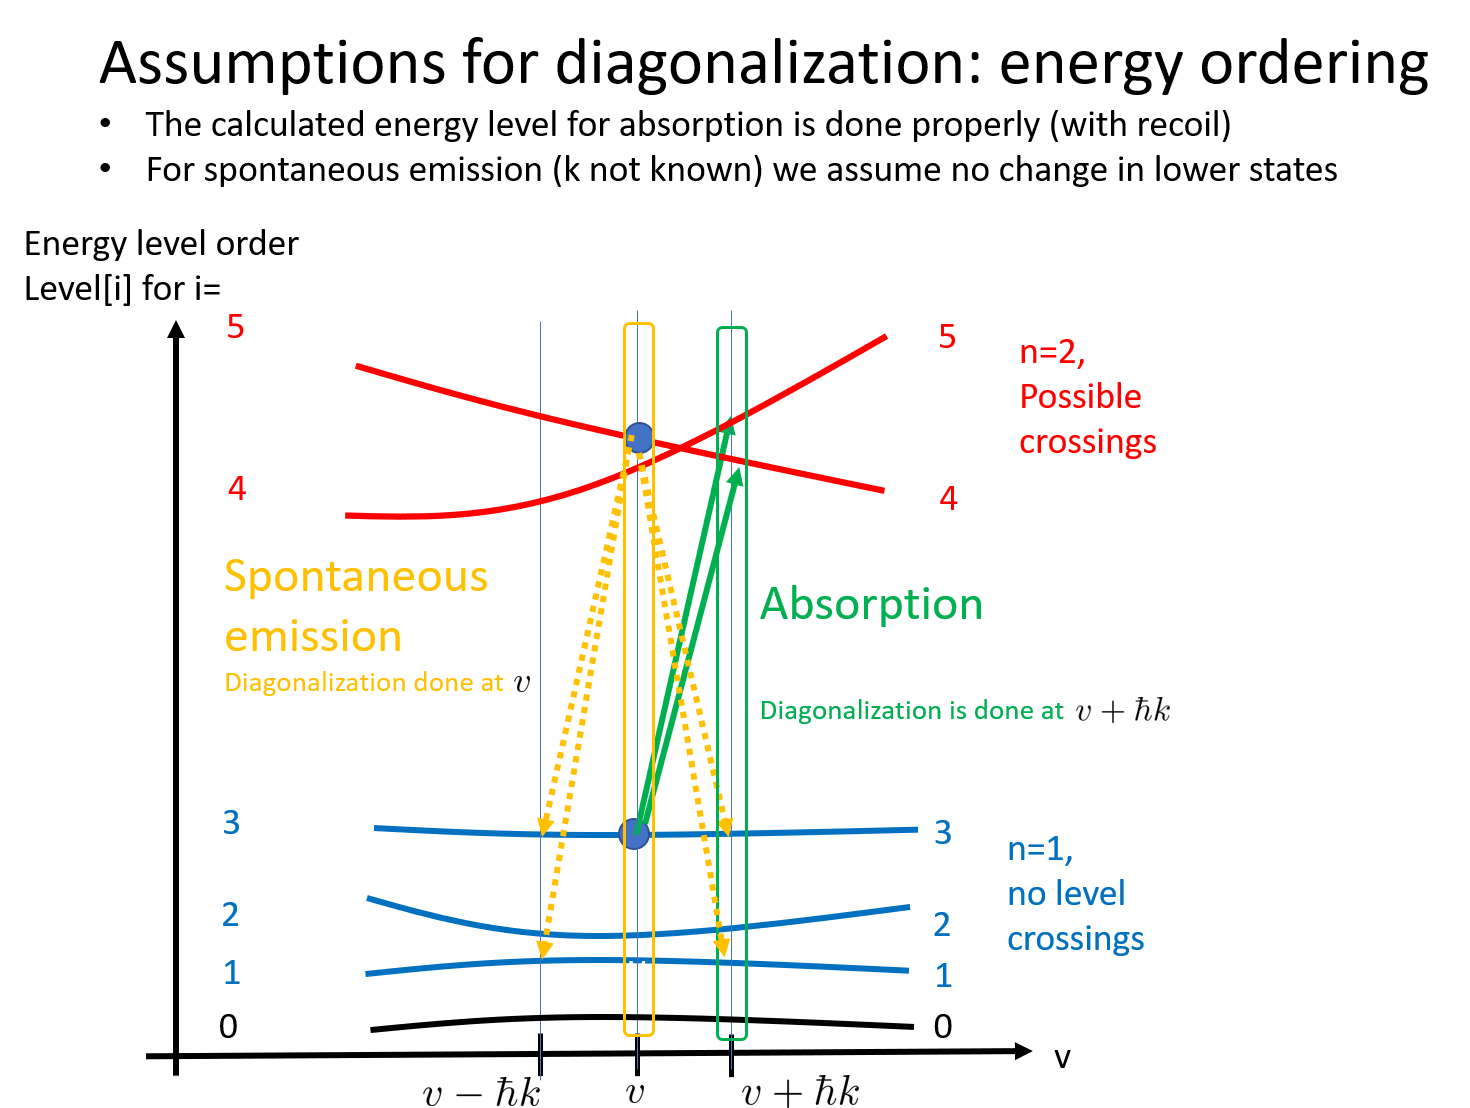
\includegraphics[width=0.6\linewidth]{diagonalization.png}
	\caption{Schematics of the Energy level due to recoil momentum. The diagonalization thus works only if the energy levels before and after spontaneous emission have the same order in energy. No other dynamical evolution is taken into account, we assume constant velocity during  motion (in the excited states).}
	\label{fig:diagonalization}
\end{figure}


The matrices (Zeeman, Stark, dipoles\footnote{From a dipole Matrix between all levels the dipole matrices could be calculated using Create\_dipole\_Lines\_from\_Matrices. And thus they are correct for the emission-absorption polarization.}) should be put by hand in diagonalization.cpp and should follow the same ordering than the Levels and Lines (and should be ascending in energies).



The most important is that in the degeneracy number \# of the state should be the number of the state staring from 0 (so Level[\#] is the Level itself) [recall that in C++ the index of the first element of the table is 0].
% The Lines file should contains all transitions (even the nul ones) between i\_low and j\_up.
The levels are thus always refers as Level[i] that is the (i+1)$^{th}$ in energy level ordering (which is not necessary the order you put originally in your level file, EXCEPT for ground state, cf FIG.{fig:diagonalization}). But, for the "sortie" or analysis Level[i] keeps its characteristics (such as M values) given in the input Level file: only Energy\_cm is updated.


% Because the magnetic $m$ quantum number, that defines the quantification of the light, is not anymore a good quantum number,  the angular emission pattern for the spontaneous emission is done isotropically.

	\subsection{Overview external versus internal dynamics}
	
We do not discuss here the Kinetic Monte Carlo (KMC) neither the N-Body solver used to solve  rate equations, this is discussed in PRA 89, 043410 (2014).
But we explain the way how code calculates the evolutions for $N$ particles, in order for interested people to modify it. 
The main part is the main.cpp file in the
 \textit{ while(velocity\_scaling == false)}
loop (before is a tentative to reach thermal equilibrium is a trap using the Berendsen thermostat Algorithm) and especially the 
\textit{ calcul\_rates\_molecules}
function.

The code calculate a time for an internal state evolution dt\_KMC (typically one over the maximal rate) and compare it to the time for the external state evolution dt\_dyn (that is now fixed and given is a parameter in the liste\_Param, even if a commented line to calculate it can by tried). 
Then the internal evolution \textit{do\_reaction} and the external \textit{evolve\_step} evolution
depends on the Choix\_algorithme\_Monte\_Carlo and Choix\_algorithme\_N\_corps parameters chosen in in Liste\_Param. 
	For instance the Choix\_algorithme\_N\_corps is commented in the Liste\_Param. This can be of importance if Coulomb interactions are present or not, or if the dipolar force is included (not well calculated for spectrally shaped laser for instance) or if we calculate it directly using gradient of the fields analytical formula (if implemented) 
	or through the potential derivative (this is the most general way fo doing it). 
	
	\subsection{Calcul (internal) rates molecules}
	
The \textit{ calcul\_rates\_molecules}
function is the most important one.

In order to not spent too much time on updating all the rates of all molecules we only recalculate the rate of the molecule (number\_mol) that has evolved internally. All others rates will be updated only after (t\_mise\_a\_jour) the dynamical (external state evolution dt\_dyn) time, so when they have moved enough to be in another environment (laser or fields intensity for instance) where the excitation-deexcitation rates have evolved.

It is possible to force some rates (like by using Pompage\_optique\_force paramter) but genearly we let the system calculate first the spontaneous emission rate and then the key function is the  \textit{ \textbf{rates\_molecule}} function.
It is quite complex but commented, here I simply mention that the local parameters such as local intensity, polarization, dipole moment $d$ etc... are calculate and the rate is calculated in \textit{ \textbf{rates\_single\_molecule\_laser\_level}} that is usually the only function that has to be modified if you want to add a new laser type (such as Black Body one).
The stimulated and absorption rate for an $i\leftrightarrow j$ transition  for a  laser of polarization vector $\bm \epsilon$ is given by $$\gamma= \frac{\pi ({\bm d}.{\bm \epsilon})^2 I_\upomega \otimes L(\omega+\bm k.\bm v-\omega_{ij}) }{\hbar^2 \epsilon_ 0 c}$$  (cf Formula (B.7) of the PRA 2014 article with the correct $\hbar^2$ factor!). So with a local intensity resulting of the convolution of the laser spectrum $I_\upomega$ with the 
transition Lorentzian $L(\delta) = \frac{\Gamma_{ij}}{2\pi}\frac{1}{\left( \frac{\Gamma_{ij}}{2}\right)^2 + \delta^2}$.

For instance for a laser with a Lorentzian spectrum of FWHM $\Gamma_L$ we have, for the Doppler induced detuning $\delta = \omega+\bm k.\bm v-\omega_{ij}$, the rate:
$\gamma=
I \frac{\pi ({\bm d}.{\bm \epsilon})^2  }{\hbar^2 \epsilon_ 0 c}
<<<<<<<< Updated upstream:User Guide/User Guide Laser Cooling_old.tex
 \frac{\Gamma_{ij}+\Gamma_L}{2\pi}\frac{1}{\left( \frac{\Gamma_{ij}+\Gamma_L}{2}\right)^2 + \delta^2}$  where $I= \varepsilon_0 E^2 c /2$ is the total laser irradiance (intensity).

========
 \frac{\Gamma_{ij}+\Gamma_L}{2\pi}\frac{1}{\left( \frac{\Gamma_{ij}+\Gamma_L}{2}\right)^2 + \delta^2}$  where $I= \varepsilon_0 E^2 c /2 = \int I_\upomega (\omega) {\rm d} \omega$ is the total laser irradiance (intensity).
 
 
This last formula helps also to understand how to treat bound-bound and bound-free rates in a similar manner because at resonnance
$\gamma = \frac{\Omega_{ij}^2}{\Gamma_{ij}+\Gamma_L} = 4 \pi^2 \alpha \frac{d_{ij}^2}{e^2} \frac{2 I}{\hbar (\Gamma_{ij}+\Gamma_L)} $ whereas for a photoionization we find 
$\gamma  = 4 \pi^2 \alpha \frac{d_{ij}^2}{e^2} \frac{ 2 I}{E_h} $ like if it was a  bound-bound transition but  with a "linewidth" given by the Rydberg constant $E_h/2$.
>>>>>>>> Stashed changes:User Guide/User_Guide_Laser_Cooling_v2.4.tex


	\subsection{Calcul (external) motion}

The \textit{ evolve\_step} is the function that evolves the external degree of freedom depending on the chosen algorithm (Verlet, Boris, ..) and most important on the way we calculated the force. We can use directly the acceleration or the derivative of the potential (depending on the choix\_epsilon parameter typically 10nm).
The fastest is clearly the use of the acceleration calculate in the 
 the key function is the  \textit{ \textbf{new\_acc}} function. But this require that the gradient of the fields are analytically calculated. This is not the case for the dipolar potential neither if there is $N$ body interaction where in this case algorithm use the gradient of the potential to calculate the force through the  \textit{ \textbf{new\_pot}} function. The dipolar potential requires to calculate all dipolar transitions (so it calls the rates\_molecule function) and this might be very slow!
 

 \subsection{Comments}
 
The code has evolved and because it is time consuming ot keep all the time the internal Energy of the molecule correct (especially if dipolar potential is used) we do not use anymore the
set\_pot\_all\_mol function and and we therefore do not 
the Internal\_state.Energy\_cm is not correct. It should not be used but (see  rates\_molecule) recalculated when needed.

In order to avoid gigantic storage we have single Levels and Lines files and ALL particles point to this and only the Zeeman , Stark and dipolar shift are added to this. For more complex situation where the internal state quantum numbers are modified for instance we need to use the Levels\_Lines\_Diagonalized 

	\subsection{Levels Lines Diagonalized }
This is controled using the is\_Levels\_Lines\_Diagonalized parameter

	\section{Performance test}
	
	 N=100 Hydrogen atoms during 50 microsecond and plot every microsecond.  64.571s with graphics versus 57.502 without and 55.826 without any output (depending on what the computer is doing meanwhile those times can fluctuate within few percent).
	 
	 
	 \subsection{Nb of molecules}
	 
	 \begin{tabular}{|c|c|}
	 	\hline
Time & Nb atoms \\
\hline
\hline
0.632 & 1 \\
\hline
	 6.984 & 10  \\
	 \hline
	26.362  & 50 \\
	 57.502 & 100 \\
	 \hline
	\end{tabular}

	 So the code is very linear in $N$ which is good news ! This is because the particle are not charged if not probably (to be tested) the variation will be in $N^2$.
	 
	  \subsection{Kinetic Monte Carlo algorithm}
	  
It is be interested to compare them (cf
	  	https://en.wikipedia.org/wiki/Kinetic\_Monte\_Carlo)
	  	because the default one 
	  	Kinetic\_Monte\_Carlo
	  	is not the fastest in principle but First\_Reaction\_Method
	  	is also perfect as well as Random\_Selection\_Method if the rate are time independent.
	  	
	  
	
	 
	 \begin{tabular}{|c|c|}
	 	\hline
	 	Time & Algorithm \\
	 	\hline
	 	\hline
	 	58.604 & Kinetic Monte Carlo (0) \\
	 	\hline
	 	132.343 & Random Selection Method (1)  \\
	 	\hline
	 	73.606  & First Reaction Method (2) \\
	 		\hline
	 	6.118 & Fast Rough Method (3)  \\
	 	\hline
	0.537 	 &  No laser included \\
	 	\hline
	 \end{tabular}
 
	 So Fast Rough Method (to be tested in more detail) may be a good way to start.
	 
Random Selection Method  has probably a problem in the code to be this slow!
	 
	 
	 
	 \subsection{Motion algorithm}
	 
	 for dt\_dyn\_epsilon\_param = $10^{-7}$ the time (for 100 atoms) is  57.502s whereas for  $10^{-8}$ the time  is  72.933s. Always choix epsilon is 1e-8.
	 
	 For 1e-7 we made test of the algorithm. Obviously the accuracy of higher order are better so dt\_dyn\_epsilon\_param can be reduced if using such algorithm but this gives an idea.
	 
	 	 \begin{tabular}{|c|c|}
	 	\hline
	 	Time & Algorithm \\
	 	\hline
	 	\hline 
	 	\\
	44.639 &	Aucun N corps (-1) \\
	 	\hline
	49.647	& Verlet acc  (sans force dipolaire) (1) \\
	 	\hline
	 252.635	&Verlet pot (avec potentiel dipolaire) (2)  \\
	 	\hline
	 86.587 & Yoshida6 acc (3) \\
	   \hline
	113.549  & Yoshida6 pot (4)  \\
	 	\hline
	474.885 	& Verlet pot gradient high order (6)
	 	\\
	 	\hline
	 49.341	& Boris Buneman  (with Magnetic field for charged particles) \\
	 	\hline
	 \end{tabular}
	 
	 
	 
	 
	 \section{Futur}
	 Despite the fact that the code could largely be improved to use more C++ spirit (like maps between reaction and rates, ...), a long list of possible improvements exists among them are:
	 
	 \begin{itemize}
<<<<<<<< Updated upstream:User Guide/User Guide Laser Cooling_old.tex
========
	 	

>>>>>>>> Stashed changes:User Guide/User_Guide_Laser_Cooling_v2.4.tex
	
	 	\item Use of adaptive time steps (like t\_evol\_ext) for the algorithms.
	 	
	 	\item Possibilities to use more general laser beam (Laguerre Gauss, others polarizations). 	Put the Gouy's type of  phase given by the polarizations.
	 	
	 	\item Optimize the link between the renew of the rates, the KMC steps and the external evolution steps. For instance if the acceleration is known we do not need to recalculate each time in the evolution algorithms ...
	 	
<<<<<<<< Updated upstream:User Guide/User Guide Laser Cooling_old.tex
	 	\item Parallelization of the code. Using  OpenMP for multiprocessor seems quite easy: If needed, download the last MinGW 64bits version.
	 	Copy-paste and erase the old one in Codeblock directory. Then in Global Compiler setting (or simply in your project) use in Other option -fopenmp.
	 	Linker settings: Adds the MinGW/bin libgomp-1.dll. Then test using simple program
	 	with \# include <omp.h>
	 	+ \# pragma omp parallel
	 	
	 	
	 	\item Combine electric and magnetic field of arbitrary orientations. This is partially done using the diagonalization cf section \ref{diagonalization}
========
	 
	 
>>>>>>>> Stashed changes:User Guide/User_Guide_Laser_Cooling_v2.4.tex
	 	
	 	\item Treat chemical reactions during collisions.
	 	
	 	\item Treat coherent dark states by choosing the proper basis.
	 	
	 	\item Use an ionization or photodetachment cross-section which is dependent on the energy.
	 	
	 	\item For strongly focused lasers, we can put the local wave-vector $\bf k$, not the global one as it is now.
	 	
	 	\item Draw lasers using the hyperbolic function (nor the elliptic one).
	 	
	 	\item Improve the statistical initial distribution. Until now we calculate the trapping field using a linear approximation for the potential energy.
	 	
	 	\item Improve the calculation of the dipolar shift. Until now the dipolar potential is not included in the shift for the transition. This avoids accumulation, but in some cases, it may be good to have it.
	 	
	 	\item Improve performance using GNU Gprof (Code Profiler Pluggin in Code::Blocks)
	 	
	 	
	 \end{itemize}
	 
	 
	 
	 \newpage
	 
	 \appendix
	 \section{Use of Pgopher}
	 
	 As mentioned before you can use Pgopher (pgopher.chm.bris.ac.uk/) to create your input files. It is in fact recommended because they have been written from it.
	 
	 Be sure to have a good simulation. For instance for a single pair of equivalent nuclei (such as in I$_2$) the statistical weights should  be SymWt=1, AsymWt = 0, rather than both 1.
	 Be sure to have enough J but not too much to avoid too big files...
	 
	 So read carefully Pgopher manual.
	 
	 Then in the Pgopher data use the following options. Hopefully with obvious notations:
	 
	 \begin{itemize}
	 	\item 
	 	MIXTURE:
	 	Precision 12
	 	
	 	QuantumNumberFormat 2J. But be careful that  all values such as tensor rank, max J are thus doubled, so it is sometimes difficult to follow them. So it is better to do this only at the end, it is just use to produce the "Levels" and "Lines" files.
	 	
	 	BField 1e-10.    In order to separate M levels and have all transitions!
	 	
	 	\item SIMULATION:
	 	IntensityUnits: EinsteinA (to have the rate for spontaneous emission)
	 	
	 	
	 	\item SPECIES:
	 	ShowJ, ShowOmega, ShowN, ..  all TRUE
	 	
	 	
	 	
	 	\item TO PRODUCE THE "LINES" FILE: Use the following option
	 	File Export Line List .txt (tab separation). Intensity Threshold 1e-8. No "Fit File Format"
	 	
	 	
	 	\item TO HAVE THE ENERGY LEVELS IN FIELDS:
	 	
	 	View, Levels List (To have the energy at each points). Verify to have All symmetry, Omega M values ...
	 	Then use "Track State" and click on "Summary". This gives levels + fit linear + quadratic of the field dependence. So be careful to plot with the proper B field T values (0-1T or 0-1mT for instance)
	 	Save the file in LEVEL.
	 	
	 	
	 	
	 	\item THEN GO TO ORIGIN (http://www.originlab.com/) or to any other data acquisition software  (in the Directory Data: Pgopher\_Level\_List.opj) and follow the following procedure.
	 	
	 	Your  case can be slightly different if you have more molecules or several vibrational levels or .. so adapt it!
	 	
	 	
	 	\begin{itemize}
	 		
	 		
	 		\item  To produce the "LEVELS" file:
	 		
	 		Remove the \%  from the LEVEL file
	 		
	 		Use Import Wizard in Origin  with 11 headers, 1 subheader (should be recognized).
	 		The name of the columns should be (if not modify  by coping this line, or use the example in):
	 		
	 		Molecule	Manifold	2M	Sym	\#	g	Population	Label	State	2J	2N	2Omega	Fn	parity*M	Energy	Linear	Dipole	Err	Quadratic	Err 2\_Level	Delta	C	Dipole2	Err	
	 		
	 		
	 		Sometimes Pgopher does not create the first column Molecule neither the last columns of E\_2\_Level ...
	 		
	 		
	 		Then we have to calculate the C and $\Delta$ (that is Delta)  coefficients when they are not given, that is if Level Delta C Dipole2 Err columns are missing. 
	 		If the effect is not linear but quadratic or more complex then  create the 2\_level fit by: 
	 		Add one column for numbers,
	 		Sort by 2\_Level.
	 		For those who do not have a 2\_Level then create one (for instance take the Linear and the same energy because C=Lin�aire, Delta=0). The  intermediate case between linear and quadratic is more complex and an appropriate formula should be derived.
	 		Sort again (a priori the file is sort in  M, Sym and \#). It is also possible to sort in Energy
	 		
	 		Duplicate the workbook  and  keep only the following columns (v is State):
	 		
	 		Manifold	2M	Sym	\#	population  	v 	2J	2N	2Omega	Energy	Delta	C
	 		
	 		
	 		Remark: One possibility to remove "v=" that appears when exporting from Pgopher in "State" and to keep only the vibrational level value is: after the  exportation  remove "v=" (and change "," in "." if needed) and import again.
	 		
	 		Then use only values not the text, so:
	 		In Manifold use 0 for the X state (lower) et 1, 2, ... for higher  Manifold and
	 		+/-1 for Sym.
	 		
	 		If wanted you can sort the workbook in Energy and modify the population column to put the desired one.
	 		Export the Workbook without headers (no Label) and in a file with .dat extension
	 		
	 		Check that the decimal are with "." not "," 
	 		Remove the space at the end of the file.
	 		
	 		
	 		
	 		
	 		
	 		\item  TO PRODUCE THE "LINES" file:
	 		
	 		Remove the first and last 2 lines of the file LINES.txt
	 		Import it in Origin (using options: delimator, Tab/space).
	 		Change the name  of the lines: (copy paste the one below)
	 		
	 		Molecule	Upper Manifold	2M'	Sym'	\#'	Lower Manifold	2M"	Sym"	\#"	Position	Intensity	Eupper	Elower	Strength	A	Width	Branch	LabelUpperManifold	state	2J'	2N'	2Omega'	Fn'	2M'	Sym	Upper Manifold	state	2J''	2N''	Omega''	Fn''	2M''
	 		
	 		
	 		Duplicate the workbook and keep only the columns:
	 		
	 		UpperManifold	2M'	Sym'	\#'	LowerManifold	2M"	Sym"	\#"	Position	Intensity	Eupper	Elower	Strength 	
	 		
	 		then do the same as for Levels: X=0, Sym =+/-1 ...
	 		
	 		Finally divide by 3 the Strength column and export in .dat file
	 		
	 	\end{itemize}
	 	
	 \end{itemize}
	 
	 
	 	 \section{Detail of laser interaction}

The code is based on \cite{comparat2014molecular};  on \cite{chaneliere2018phase} (supplementary material) for quantization, recoil and Doppler effects;  and on
\cite{manual_Steck,varshalovich1988quantum} for vector and angular momenta.
We recall here some important points. The notations differ sometimes from  \cite{comparat2014molecular}  but are more general  and should be preferred, because we use less assumptions here (especially about the reality of some vectors).
	 	 
	 	  	 
	 	 \subsection{Spherical  and helicity vectors }
	 	 
	 	 We  use the notation of \cite{varshalovich1988quantum} such as the (covariant) spherical  vectors 
	 	 $ {\bf e}_0 = {\bf e}_z, {\bf e}_{\pm 1} =  \mp \frac{{\bf e}_x \pm
	 	 	i {\bf e}_y} { \sqrt{2}}$.
	 	 Using ${\bf{e}}^q = ({\bf{e}}_q)^* = (-1)^q {\bf{e}}_{-q}$ (that leads to the normalization ${\bf{e}}^p  {\bf{e}}_q = \delta_{pq} $) we find for any (complex) vector
	 	 $$\bm A = \sum_q A^{q} {\bf{e}}_q  = \sum_q (-1)^q A_{-q} {\bf{e}}_q   $$
	 	 where 
	 	 $A_q = \bm A.
	 	 {\bf{e}}_q$ so for instance $A_0 = A_z, A_{\pm 1} =  \mp (A_x \pm
	 	 i A_y)$.
	 	 %	If $\bm A$ is a \textit{real} vector we have $\bm A = (\bm A)^*$ and $ A^q = A_q^*$ so $\bm A =  \sum_q  A_q^* {\bf{e}}_q  	$.
	 	 We will often have the case where the $A_q$ or $A^q$ are reals (example of the dipoles or of pure laser polarization) but in general we should keep in mind that the vectors are complex.
	 	 
	 	 
	 	 
	 	 \subsection{Lasers using  complex notations}
	 	 
	 	 
	 	 
	 	 
	 	 The electromagnetic field, due to the lasers $\rm L$, can be written
	 	 $${\bm E}(\bm r,t) = 	 {\bm E'}(\hat{\bm r},t)+ {\bm E'}^\dag(\hat{\bm r},t)  = \frac{1}{2}\sum_{\rm L}    \left[ {\bm E}_{\rm L} e^{i(  {\bm k}_{\rm L}. {\bm r} - \Phi_{\rm L}
	 	 	(t))} +  {\bm E}_{\rm L}^\ast e^{-i(  {\bm k}_{\rm L}. {\bm r} - \Phi_{\rm L}
	 	 	(t))}  \right] $$
	 
	 	 the irradiance, called improperly  intensity, is 
	 	$
	 	 I_{\rm L}= \varepsilon_0 |E_{\rm L}|^2 c/2 $.
	 	 
	 	 
	 	 
	 	 The Doppler effect, and the laser linewidth, are taken into account by writing $\Phi_{\rm L} (t) = (\omega_{\rm L}  - {\bm k}_{\rm L}. {\bm v}) t + \Phi^{\rm L} (t)$. Where $\Phi^{\rm L} (t) $ is  a fluctuating phase. 
	 	 
	 	 
	 	As shown in Fig. \ref{fig:laseraxispolarization},
	 	  we   use  the (covariant polar basis) frame linked with the laser propagation:
	 	$({\bf{e}}'_{\rm x} = {\bf{e}}_{\theta} , {\bf{e}}'_{\rm y} = {\bf{e}}_{\phi},  {\bf{e}}'_{\rm z} = {\bf{e}}'_{\rm r} = \bm{k}/\| \bm{k} \|)$ . 
	 	  The  laser polarization is  conveniently described in the (covariant) helicity basis
	 	 $ {\bf e}'_0 = {\bf e}'_z,  {\bf e}'_{\pm 1} =  \mp \frac{{\bf e}'_x \pm
	 	 	i {\bf e}'_y} { \sqrt{2}}$.
	 	 For each laser $\rm L$
	 	 the polarization vector, defined by 
	 	 $ {\bm E}_{\rm L}(\bm r,t) = E_{\rm L}(\bm r,t) {\bm \epsilon}_{\rm L} $, is  $ {\bm \epsilon}_{\rm L} =
	 	 \sum_{p= -1,0,+1} \epsilon'^p 
	 	 {\bf e'}_{p}  $.
	 	 
	 
 In the code we deal (for simplicity and for calculus speed) only with reals. So for instance
	   	 \textbf{the polarisation is  coded using only 3 real parameters  Pol\_circulaire\_right\_sm ($a_{-}$), Pol\_circulaire\_left\_sp ($a_{+}$)  and polar\_angle\_degree  ($\Psi$) (in degree in Liste\_Param). These 3 parameters
 define 
	 \begin{equation}
	 {\bm \epsilon}_{\rm L} = {\rm Pol\_circulaire\_right\_sm} \ e^{i \Psi} {\bf e'}_{-1} + 	 {\rm Pol\_circulaire\_left\_sp} \ e^{-i \Psi}
	 {\bf e'}_{+1} =   a_{-} \ e^{i \Psi} {\bf e'}_{-1} + 	a_{+} \ e^{-i \Psi}
	 {\bf e'}_{+1}  
	 \end{equation}}
	  % ${\bf{e}}'_{\rm L,pol} = \{  Pol\_circulaire\_right\_sm = \epsilon'^{-1} e^{-i \Psi}, \epsilon'^0 , Pol\_circulaire\_left\_sp = \epsilon'^{+1} e^{i \Psi} \}$	
	  
	 This does not authorize arbitrary polarizations but only pure circular (right with  $\epsilon'^{-1} =1$, or left with $\epsilon'^{+1}=1$) or
	 a pure linear polarization. For example,   (cf. Fig.
	 \ref{fig:laseraxispolarization}) linear polarization turned by an angle $\Psi$ from $ {\bf e'}_{x} $
is  ${\bm \epsilon}_{\rm L} = {\bf e}'_x \cos\Psi + {\bf e}'_y \sin \Psi = 
	  \frac{1}{\sqrt{2}} e^{i \Psi} {\bf e'}_{-1} - 	 \frac{1}{\sqrt{2}} e^{-i \Psi}
	  {\bf e'}_{+1}  $, that is $a_{-} = \frac{1}{\sqrt{2}}, a_{+}= - 	 \frac{1}{\sqrt{2}}$.	  
	  % and is thus   ${\bf{e}}'_{\rm L,pol} = \{ 	 \frac{1}{\sqrt{2}} e^{i \Psi}, 0 ,  - 	 \frac{1}{\sqrt{2}} e^{-i \Psi} \}$ which is not real.
	  
	
	 	 
	 	 \subsection{Transition dipole moment}
	 	 

	 	 
	 	 The transition dipole moment 
	 	 ($\bm d = e \bm r$ in the simple case of H, Ps or alkali atoms, and we will use often this simplification for the notation)
	 	 between 2 levels is defined (for now in the lab fixed frame but this will be precised in section \ref{pol_vector})  as
	 	 $ \bm d_{ij} = \langle i | \bm d | j \rangle = \sum_q (-1)^q d_{ij;q} {\bf{e}}_q = \sum_q d_{ij;q} {\bf{e}}^q $ so $ d_{ij;q} = \bm d_{ij}.{\bf{e}}_q$. The notation $d_{ij}^{(q)} = d_{ij;q}$ is often used but has to be avoided because of possible confusion with the (contravariant) notation $d_{ij}^{q}$.
	 	 The correct component that forms an irreductible tensor (rank 1) $\hat d_{1q} = \hat d_{q}$ are $ d_{ij;-1},d_{ij;0},d_{ij;+1} $. 
	 	 In the code this vector is called
	 	 the "polarization" dipole vector  $\bm d_{ij} $ and is recorded as $ \{ d_{ij;-1},d_{ij;0},d_{ij;+1} \} $ (obviously in C++ the array number will be respectively dipole[0], dipole[1], dipole[2]).
 With the proper (Condon-Shortley's type) convention \cite{varshalovich1988quantum}, these dipoles are reals.
	 	 
	 %	 We also	 	 the polarization dipole vector  by ${\bf{e}}_{\rm pol,ij} =  \bm d_{ij}/|d_{ij}| = 	  \{ d_{\rm pol,ij}^{-1}, d_{\rm pol,ij}^0 , d_{\rm pol,ij}^{+1} \} $
	 	
	 	 	 	 

	 	 	
	 	 
	 	 \subsection{Absorption, stimulated or spontaneous emission}
	 	 
	 	 For a transition between two states $|j\rangle$ to $|i\rangle$,  it is important to known if we deal with absorption (rising level energy) or stimulated or spontaneous emission  (lowering level energy) to know which term in the rotating wave approximation shall be used. 
	 	 
	  \textbf{	 In the following, we assume $E_j> E_i$}.
	 	
	 		 		 	 \subsubsection{Ordered energy levels and rotating wave approximation}
	 		 		 	 
	 		 		 	 
The rotating wave approximation leads (for level $j$ above level $i$: $E_j>E_i$) leads to:
	 	
	 	\begin{equation*}
	 	\hat H =  \frac{\bm \hat {\bm p}^j}{2 m} + 
	 	V_i(\hat {\bm r},t) |i\rangle\langle i| + V_j(\hat {\bm r},t) |j\rangle \langle j| 
	 	-   \langle j | q \hat {\bm r}| i \rangle .\bm E' (\hat {\bm r} ,t)  |j\rangle \langle i| -  \langle i | q \hat {\bm r}| j \rangle .  \bm E'^\dag (\hat {\bm r} ,t)  |i\rangle \langle j| \label{hamiltonianRWA}
	 	\end{equation*}
	 
	 	where we have added some  potential traps $V_i$ and $V_j$ to be more general.
	 %	where the coupling term is  $\displaystyle \hat V = -  \bm d .\bm E' (\hat r ,t) = 	- \frac{\bm d}{j}\sum_{\rm L}    {\bm E}_{\rm L}(t) e^{i(  {\bm k}_{\rm L}. {\hat{\bm r}} - \omega_{\rm L} t  - \Phi_{\rm L}(t) )}		= \sum_{\rm L}	\hat V_{\rm L}	$.	
	 	
	 	The recoil effect will be present only after the interaction by a $\hbar \bm k$ term added to the momentum. This is clarified, cf Eq. (9) and (20) of \cite{chaneliere2018phase}, by using the (single plane wave, in a volume $L^3$)
 quantized field:
	 	$\displaystyle	\hat{\bm{E}} (\bm{r},t)  = \sum_{\bm{k},\sigma} i \sqrt{\frac{ \hbar  \omega_k}{2  \epsilon_0 L^3} } \left(  \hat a_{\bm{k} \sigma} e^{- i \omega_k t}  \bm{\epsilon}_{\bm{k}\sigma} {\rm e}^{i \bm{k}.\bm{r} }  - \hat a_{\bm{k} \sigma}^\dag  e^{ i \omega_k t}  \bm{\epsilon}_{\bm{k}\sigma}^\ast {\rm e}^{-i \bm{k}.\bm{r} } \right)$, where $ {\bm \epsilon}_{\bm k \pm 1} =  {\bf e}'_{\pm 1}$.  We thus have:
	 	\begin{equation*}
	 	\hat H =  \frac{\hat{\bm p}^2}{2 m} + 
	 	V_i(\hat{\bm r},t) |i\rangle\langle i| + V_j(\hat{\bm r},t) |j\rangle \langle j| \label{eq_base_at}
	 	-  \bm d_{ji}. \hat{\bm E'} (\hat{\bm r} ,t)    |j\rangle \langle i| + \bm d_{ij} .{\hat{\bm E'}}^\dag (\hat{\bm r} ,t)  |i\rangle \langle j|  +
	 	\sum_{\bm{k} \sigma} \hbar \omega_k \left( \hat a^\dag_{\bm{k} \sigma} \hat a_{\bm{k} \sigma} + 1/2 \right) 
	 	\end{equation*}
	 	where  $\bm d_{ji} = \langle j | q \hat {\bm r}| i \rangle = \bm d_{ij}^* $ is the transition dipole element. The quantization  clarifies  the recoil effect because of
	 	$
	 	e^{ \pm i \bm k.\hat{\bm r}} | \bm p\rangle = |\bm p \pm \hbar \bm k\rangle$.
	 
	

	Descriptions of the rate equations and forces can be find in the appendix of Ref.  \cite{comparat2014molecular,chaneliere2018phase} and are not recalled here.
	
	 		 	
	 		 	 
	 		 	 
	 		 	
	 		 	 
	 		 	 
	 		 	 \subsubsection{Absorption, Stimulated or spontaneous emission}
	 		 	 

	 	 
	Absorption is thus a  transition $i \rightarrow j$ ($E_j> E_i$). For absorption
	 the only relevant term is due to $-\bm d.\bm E'$ through the Rabi frequency\footnote{	For more generality we do not (yet) assume real dipoles and so the notation is different (better here even if careful has to be taken in the $i,j$ order because $\Omega_{ji} =\Omega_{i \rightarrow j} $ ) than in \cite{comparat2014molecular}.}
\begin{equation}
\hbar  \Omega_{ji} = E_{\rm L} \langle j, \bm p + \hbar \bm k |   \hat{\bm d} . \bm \epsilon_L
	e^{ i \bm k.\hat{\bm r}} | i, \bm p\rangle =  E_{\rm L}   \bm d_{ji} . \bm \epsilon_L = E_{\rm L} 
 \sum_q  d_{ji;q} {\bf{e}}^q .	\sum_{p} \epsilon'^p 	{\bf e'}_{p} 
 \label{Rabi_frequancy}
 \end{equation}
	



	 	 
	 	The stimulated emission  $j \rightarrow i$  with the same laser is govern by the $-\bm d.{\bm E'}^\dag$ term and thus arises with the Rabi frequency
$\hbar  \Omega_{ij}  = E_{\rm L} \langle i, \bm p - \hbar \bm k |   \hat{\bm d} . {\bm \epsilon_L}^\dag
	 	 e^{  - i \bm k.\hat{\bm r}} | j, \bm p\rangle = E_{\rm L} \bm d_{ij} . {\bm \epsilon_L }^\dag =\hbar  \Omega_{ji}^*$
	 	 
	 	 We recover the well known fact that the dipole transition rates are the same (conjugated Rabi frequencies) for spontaneous and for stimulated emission.
	 	 
	 	 
	 	 	 The simplest (ideal) case is when
	 	 \begin{itemize}
	 	 	\item The  quantization axis and laser axis (for the polarization) are equal ${\bf{e}}_q={\bf{e'}}_q$.  In this case,  	  the absorption is driven by $\hbar  \Omega_{ji} = E_{\rm L} \sum_q  d_{ji;q}  \epsilon'^q $
	 	 	\item The laser is of pure polarization $ \epsilon'^q =1$ for a given $q$ and $0$ for others. So $\hbar  \Omega_{ji} = E_{\rm L}  d_{ji;q} $
	 	 	\item  states are pure (that is with well defined magnetic quantum numbers $m_i,m_j$ projection on the quantization axis ${\bf{e}}_0$). So $\hbar  \Omega_{ji} = E_{\rm L}  d_{ji;q}  =  E_{\rm L}   \langle j |   d_{1q} | i \rangle $ will verifies $m_j = q+ m_i  $.  We recover the fact that
	 	 	$ q=-1$ for a $\sigma-$, 	 $ q=0$ for a $ \pi$ and
	 	 	$ q= +1$ for a $\sigma+$ light. 
	 	 \end{itemize}
	 	
	 	 
We now have to treat the most general case where none of these 3 assumption is correct.
	 	 	 	 \subsection{Rotation matrices}
	 	 	 	
	 	 	 	We have to deal with three frames:
	 	 		 	 \begin{itemize}
	 	 	 		\item The fixed lab frame 	$(\bf{e}_{\rm x},  \bf{e}_{\rm y},  \bf{e}_{\rm z}  )$ 
	 	 	 		\item The local (different for each particle position $\bm r$) field $\bm F(\bm r)$ frame, 	$(\bf{e}_{\rm X},  \bf{e}_{\rm Y},  \bf{e}_{\rm Z})$. It defines the quantization axis. It  will also be noted
	 	 	 				$(\bf{E}_{\rm X},  \bf{E}_{\rm Y},  \bf{E}_{\rm Z} = \bm{F}/\| \bm{F} \|)$ in order to define ${\bf{E}}_{\pm 1}$ without any  confusion with  ${\bf{e}}_{\pm 1}$.
	 	 	 		\item The laser  frame	$(\bf{e}'_{\rm x},  \bf{e}'_{\rm y},  \bf{e}'_{\rm z} = \bm{k}/\| \bm{k} \|)$.
	 	 	 	\end{itemize}
	 	 	 These frames are defined  by their $z,z',Z$ axis, and the angle of rotation around this axis is defined such  that (cf Fig.
	 	 	 \ref{fig:laseraxispolarization}), taken the example of the laser $z'$ frame, the frame is the polar frame of which $Oz'$ is the direction and $Ox'$ is the meridian.
	 	 	 	
	 	 	 	
	 	 	 	All this explain that in the code a reaction is coded using the   type\_codage\_react reaction=$\{n\_mol; n\_laser; \bm F; \bm \epsilon_L; \bm k; final\_internal\_state\}$ for the particule number $n\_mol$, under the laser number $n\_laser$ (-1 for spontaneous emission).
	 	 	 
	 	 	 	 	\subsubsection{Euler angles}
	 	 	 	 	
	 	 	 	 	To go from one 	$(\bf{e}_{\rm x},  \bf{e}_{\rm y},  \bf{e}_{\rm z}  )$  frame to a new one $(\bf{e}'_{\rm x},  \bf{e}'_{\rm y},  \bf{e}'_{\rm z} )$ it is convenient to use the  Euler angles.
	 	 	 	Different conventions exists: Mathematica and  \cite{varshalovich1988quantum} (1.4 schema A) are in the so called z y z (noted also Z Y Z) convention, whereas Wikipedia is in z x z convention. For completeness, we thus recall  here the
	 	 	 	 Euler rotations  angles	 $(\alpha,\beta,\gamma)$ convention. 
	 	 	 	 For instance in the 
	 	 	 	 	z y z convention:
	 	 	 	 	\begin{itemize}
	 	 	 	 		\item  	 	 the first rotation is by an angle $\alpha$ about the $z$-axis.
	 	 	 	 	\item the second rotation is by an angle $\beta$  about the new $y$-axis
	 	 	 	 	\item the third rotation is by an angle $\gamma$  about the new $z$-axis (now $z'$).
	 	 	 	 	\end{itemize}
 	 	 	 	
 	 	 	 	 Clearly (Fig.
 	 	 	 	 \ref{fig:laseraxispolarization}) our convention to use 
 	 	 	 	the spherical basis leads simply to 
 	 	 	 	$(\alpha,\beta,\gamma) = 	(\phi,\theta,0)$  in the 
	 	z y z convention, but to  $(\alpha,\beta,\gamma) = 	(\phi+\pi/2,\theta,-\pi/2)$ in the  z x z  convention.
	 	
	 	 The z x z convention is the one used (for historical reason) in the code (cf Euler\_angles function).
	 	 The z x z  convention is useful to find the polar angle $\phi,\theta$ knowing only the vector ${\bf{e}}'_{\rm z} = x_e {\bf{e}}_{\rm x} + y_e {\bf{e}}_{\rm y} + z_e {\bf{e}}_{\rm z}  $ that defines the new frame  by:
	 	  $\alpha = \phi+\pi/2 = {\rm atan2}(x_e, - y_e)$ and  $\beta = \theta =  \arccos(z_e)$.
	 	  
	 	  The main function in the code is thus rotation\_axis\_lab   that calculates, 	 	using simple notation such as $s_1 = \sin (\alpha)$ or $c_3 = \cos (\gamma)$  ,  the new coordinates
	 	 $$ \begin{pmatrix} x \\ y \\ z
	 	 \end{pmatrix}
	 	  =\begin{pmatrix}c_{1}c_{3}-c_{2}s_{1}s_{3}&-c_{1}s_{3}-c_{2}c_{3}s_{1}&s_{1}s_{2}\\c_{3}s_{1}+c_{1}c_{2}s_{3}&c_{1}c_{2}c_{3}-s_{1}s_{3}&-c_{1}s_{2}\\s_{2}s_{3}&c_{3}s_{2}&c_{2}\end{pmatrix}.  \begin{pmatrix} x' \\ y' \\ z'
	 	  \end{pmatrix}$$
	 	 	The reverse rotation\_lab\_axis is  used to find the laser intensity (cf intensity\_lab\_axis function) at the particle location $\bm r  = x {\bf{e}}_{\rm x} + y {\bf{e}}_{\rm y} + z {\bf{e}}_{\rm z}  $.
 	 	 	\subsubsection{Polarization vectors}
 	 	 	\label{pol_vector}
	 	 
	 	% We	 can write the laser polarization vector in the two frames  as \cite{varshalovich1988quantum} Eq. 1-(49):	 	 $ {\bm \epsilon} = 	 \sum_{p'= -1,0,+1} {\epsilon'}^\ast_{p'}  	 {\bf e'}_{p'} =  \sum_{p= -1,0,+1} \epsilon_p^\ast  	 {\bf e}_{p} $, with 	 $ \epsilon_{p} = 	 \sum_{p' =0,\pm 1 } (-1)^{p'} \epsilon'_{p'} 	 D_{p p'}^{\ast (1)} (0,\theta,\varphi)$.
	 	 
	 	To evaluate Eq. \ref{Rabi_frequancy} we
	 	  write the laser polarization vector in the three frames  	
 $ {\bm \epsilon}_{\rm L} =
	\sum_p \epsilon'^p 
	{\bf e'}_{p}  = 	\sum_p \mathcal{E}^p
	{\bf E}_{p} = \sum_p \epsilon^p
	{\bf e}_{p}
	$.
	Using  $ {\bm \epsilon}^. = \begin{pmatrix} \epsilon^{-1} \\ \epsilon^{0} \\ \epsilon^{+1}
	\end{pmatrix},   {\bm e}_. = \begin{pmatrix} 	{\bf e}_{-1}  \,	{\bf e}_{0}  \,	{\bf e}_{+1}
	\end{pmatrix}, 
	{{\bm \epsilon}'}^. = \begin{pmatrix} {\epsilon'}^{-1} \\ {\epsilon'}^{0} \\ {\epsilon'}^{+1}
	\end{pmatrix} = \begin{pmatrix}a_{-} \ e^{i \Psi}  \\ 0 \\ a_{+} \ e^{-i \Psi}
	\end{pmatrix} ,   {\bm e}'_. = \begin{pmatrix} 	{\bf e'}_{-1} \, 	{\bf e'}_{0} \,	{\bf e'}_{+1}
	\end{pmatrix}, 
	{\mathcal{\bm  E}}^. = \begin{pmatrix} \mathcal{E}^{-1} \\ \mathcal{E}^{0} \\ \mathcal{E}^{+1}
	\end{pmatrix},   {\bm E}_. = \begin{pmatrix} 	{\bf E}_{-1} \,	{\bf E}_{0} \,	{\bf E}_{+1}
	\end{pmatrix}$ we have 
	 $ {\bm \epsilon}_{\rm L} = {\bf e'}_. {\bm \epsilon'}^.   =   {\bf E}_. \mathcal{\bm E}^. =  {\bf e}_. {\bm \epsilon}^.  $

	
	
	We will note $\phi_{\bm k},\theta_{\bm k}$ the polar angles of ${\bm k}$ (to go from the lab fix frame to the laser  frame) and  $\phi_{\bm F},\theta_{\bm F}$ the polar angles of ${\bm F}$ (so to go from the lab frame to the field  frame). Eq. (1.1 53)  of Ref.
	\cite{varshalovich1988quantum} gives
	$ \sum_p	{\bf e}_{p}  {\rm  D}_{p p'}^{1} (\phi_{\bm k},\theta_{\bm k},0)  = {\bf e'}_{p'} $
that is 		
$	{\bf e}_. {\rm {\bm D}} (\phi_{\bm k},\theta_{\bm k},0)  = {\bf e'}_. \mbox{ and similarly } {\bf e}_. {\rm {\bm  D}} (\phi_{\bm F},\theta_{\bm F},0)  = {\bf E}_. $
	 where
	  $({\rm {\bm  D}})_{ij} = {\rm  D}_{i j}^{1} $ is the
	WignerD function.
	 Several conventions exists: Mathematica 
	WignerD$[\{j,m_1,m_2\},\alpha, \beta, \gamma]= {\rm  D}_{m_1,m_2}^j	(-\alpha, -\beta, -\gamma)$ of 	\cite{varshalovich1988quantum}. We use the  \cite{varshalovich1988quantum} concention, that is also the one chosen by Wikipedia with:	
	 $ {\rm {\bm  D}}  (\phi,\theta,0) =
	\begin{pmatrix}
	\frac{1}{2} e^{i \phi} (1+\cos \theta) &\frac{e^{i \phi} \sin \theta}{\sqrt{2}}  & e^{i \phi} \sin^2(\theta/2) \\
	-\frac{\sin \theta}{\sqrt{2}}	& \cos \theta	&  \frac{\sin \theta}{\sqrt{2}}	\\
	e^{-i \phi}  \sin^2(\theta/2)  & -\frac{e^{-i \phi} \sin \theta}{\sqrt{2}}  &  \frac{1}{2} e^{-i \phi} (1+\cos \theta) \end{pmatrix}
	$ with the order $i,j = -1,0,1$ in the lines and columns.
	
 Because the states $|i\rangle$ are defined with the quantization axis frame ${\bf{E}}_.$ we note
	 $ \bm d_{ij} = \langle i | \bm d | j \rangle  = \sum_q D_{ij;q} {\bf{E}}^q $ with $ D_{ij;q} = \bm d_{ij}.{\bf{E}}_q$. So in matrix notation, with
$	 {\bm D_{ij}}_.  = \begin{pmatrix}D_{ij;-1} \, D_{ij;0} \, D_{ij;+1} \end{pmatrix}  = \begin{pmatrix}D_{-1} \, D_{0} \, D_{+1} \end{pmatrix}   $ 
	and $ {\bm E}^. = \begin{pmatrix} 	{\bf E}^{-1} \\	{\bf E}^{0} \\	{\bf E}^{+1}
	\end{pmatrix}$, we have 
	$\bm d_{ij} =  {\bm D_{ij}}_. {\bf E}^.  $
 
	 	We can thus now write Eq. \ref{Rabi_frequancy} as
	 	 \begin{equation}
	 	 \hbar  \Omega_{ji} /  E_{\rm L}  = \bm d_{ji} . \bm \epsilon_L =  [ {\bm D_{ij}}_. {\bf E}^.  ].[ {\bf e'}_.  {\bm \epsilon'}^. ]
	 	% =	  [{\bm D_{ij}}_. {\bf E}^. ].[	 {\bf E}_. 	{\rm {\bm  D}}^{-1} (\phi_{\bm F},\theta_{\bm F},0) 	 {\rm{ \bm  D}} (\phi_{\bm k},\theta_{\bm k},0)  {\bm \epsilon'}^.    ]
	   =  {\bm D_{ij}}_. 	{\rm {\bm  D}}^{-1} (\phi_{\bm F},\theta_{\bm F},0) 
	 	 {\rm{ \bm  D}} (\phi_{\bm k},\theta_{\bm k},0)  \begin{pmatrix}a_{-} \ e^{i \Psi}  \\ 0 \\ a_{+} \ e^{-i \Psi}
	 	 \end{pmatrix}  
	 	 \end{equation}
	 	 
	 	 	 This formula is used in the code in the effectif\_dipole\_local function and the final result is 	 
	  \begin{eqnarray*}
	 	& & 	 \hbar  \Omega_{ji} /  E_{\rm L}  =   \frac{1}{4} e^{-i
	 		(\psi +{\phi_{\bm F}}+{\phi_{\bm k}})} \times \\
	 	&  & \Big[   \cos ({\theta_{\bm k}}) \left(-{a_+}+{a_-}
	 	e^{2 i \psi }\right) \left(\left(e^{2 i {\phi_{\bm F}}}+e^{2 i
	 		{\phi_{\bm k}}}\right) \left(\sqrt{2} {D_0} \sin ({\theta_{\bm F}})+({D_-}-{D_+}) \cos ({\theta_{\bm F}})\right)-({D_-}+{D_+}) \left(e^{2 i {\phi_{\bm F}}}-e^{2 i
	 		{\phi_{\bm k}}}\right)\right) \\
	 	&  & -2 \sin ({\theta_{\bm k}}) e^{i
	 		({\phi_{\bm F}}+{\phi_{\bm k}})} \left(-{a_+}+{a_-} e^{2 i \psi }\right) \left(\sqrt{2} {D_0} \cos ({\theta_{\bm F}})+({D_+}-{D_-}) \sin ({\theta_{\bm F}})\right) \\
	 	& & +\left({a_+}+{a_-} e^{2 i \psi
	 	}\right) \left(({D_-}+{D_+}) \left(e^{2 i {\phi_{\bm F}}}+e^{2 i
	 		{\phi_{\bm k}}}\right)-\left(e^{2 i {\phi_{\bm F}}}-e^{2 i {\phi_{\bm k}}}\right) \left(\sqrt{2} {D_0} \sin ({\theta_{\bm F}})+({D_-}-{D_+}) \cos ({\theta_{\bm F}})\right)\right) \Big]
	 \end{eqnarray*}	 

	 	 \subsection{Angular distribution of spontaneous emission: recoil}
	 	 
	 	 
	 	 The spontaneous emission rate  between a level $| i \rangle $ and $|j\rangle$ is given by 
	  $\Gamma =\|\rm d_{ij}\|^2 C_{{\rm Debye},s} E_{\rm cm}^3$ (function  Gamma\_Level\_from\_diagonalized\_dipole in the code). In order to properly take into account the recoil momentum we need to know the angular distribution of the emitted photon.
	 	 For this we have to go back to the calculation of the spontaneous emission rate that originates form the quantized field 
	 so from (Fermi golden rule)
	 	 $\sum_{\bm k,\pm 1} | \langle i | \bm d | j \rangle. {\bm \epsilon}_{\bm k \pm 1}|^2 =  \sum_{\bm k} \left[ \sum_p | \bm d_{ji} . {{\bm e'}_{\bm k}}_p |^2 - |  \bm d_{ji} . {{\bm e'}_{\bm k}}_0 |^2  \right] $. So by defining the
	 	 "polarization" vector of the emitted light as ${\bf{e}}_{\rm pol} = \bm d_{ji} /\|\bm d_{ji} \|$ we find  that the probability distribution, for
	 	 	the direction $\bm r = \bm k/k$ of the emitted photon, is 
 given by
	 	 $ \frac{3}{8\pi} [1-|\bm r.{\bf{e}}_{\rm pol}|^2]$, with the proper normalization (to $1$). 
	 	 We recover Eq. (1.45) (see also Eq. (7.427)) of Ref.	 \cite{manual_Steck}. In the code (get\_unit\_vector\_spontaneous\_emission function) the photon is  taken randomly (with the Von Neumann's acceptance-rejection sampling method) using this distribution. % That is in the quantization axis (field) frame  $d_{ji} {\bf{e}}_{\rm pol} = \sum_q D_{ij;q} {\bf{E}}^q $.
	 	
	 		 \subsection{Diagonalization of the states} 
	 		 
	 		
	 		In most of the cases the eigenstates themselves are not changing  during the evolution, only the energy changes. However, 
	 		as explained in section \ref{diagonalization}
	 		we have the possibility
	 		 to diagonalize the hamiltonian, for instance, to calculate Zeeman and Stark effect for the magnetic $\bm B$ and electric $\bm E$ fields more exactly. For this purpose,
	 		 we  give the bare states $|i\rangle_0$, their energies ${E_i}_0$, and the dipole transition moments
	 		 (in the Diagonalization\_Energy\_dipole function)  as three matrix $\{ \bm d0_{-1},\bm d0_{0},\bm d0_{+1} \} $   in the quantization frame (so always assuming adiabatic following)  with  $ 
	 		 (\bm d0_{q})_{ij} =
	 		 d0_{ij;q} =   {}_0\langle i | \hat {\bm d} | j \rangle_0 . {\bf{E}}_q $.
	 		 
	 		 
	 		 Then, for each local perturbation $\hat V(\bm B(\bm r), \bm E(\bm r) )$ 
	 		 (the perturbation $\hat V$ matrix is given in the  Diagonalization\_Energy function),	 		 
	 		 we diagonalized $ \hat H = \hat H_0+\hat V$ to get the new eigenvectors
	 		  $| i\rangle = \sum_{i_0} {}_0\langle i_0 |   i\rangle |i_0\rangle_0   =  \sum_{i_0} {\rm \bm evec}_{i_0 i } |i_0\rangle_0  $ with the eigenvectors matrix  ${\rm \bm evec}_{i_0 i } =
	 		  {}_0\langle i_0 |   i\rangle$. We can then calculate the new dipoles 
	 		$ \langle i | \hat d_q | j \rangle =  ({\rm \bm evec}^\dag.{\bm d0}_q.{\rm \bm evec})_{ij} $ that is coded with the dipole vector $ \{ d_{ij;-1},d_{ij;0},d_{ij;+1} \} $.
	
	 
\bibliographystyle{unsrt}
\bibliography{bibli_user_guide}



\end{document}




